\documentclass[a5paper]{article}
\usepackage[a5paper, top=8mm, bottom=8mm, left=8mm, right=8mm]{geometry}

\usepackage{polyglossia}
\setdefaultlanguage[babelshorthands=true]{russian}

\usepackage{fontspec}
\setmainfont{FreeSerif}
\newfontfamily{\russianfonttt}[Scale=0.7]{DejaVuSansMono}

\usepackage[font=scriptsize]{caption}

\usepackage{amsmath}
\usepackage{amssymb,amsfonts,textcomp}
\usepackage{color}
\usepackage{array}
\usepackage{hhline}
\usepackage{cite}
\usepackage{textcomp}

\usepackage[hang,multiple]{footmisc}
\renewcommand{\footnotelayout}{\raggedright}

\PassOptionsToPackage{hyphens}{url}\usepackage[xetex,linktocpage=true,plainpages=false,pdfpagelabels=false]{hyperref}
\hypersetup{colorlinks=true, linkcolor=blue, citecolor=blue, filecolor=blue, urlcolor=blue, pdftitle=1, pdfauthor=, pdfsubject=, pdfkeywords=}

\newlength\Colsep
\setlength\Colsep{10pt}

\usepackage{tabu}

\usepackage{graphicx}
\usepackage{indentfirst}
\usepackage{multirow}
\usepackage{subfig}
\usepackage{footnote}
\usepackage{minted}

\newcommand{\todo}[1] {
\begin{center}\textcolor{red}{TODO: #1}\end{center}
}

\sloppy
\pagestyle{plain}

\title{Глубокое метамоделирование}
\author{Юрий Литвинов\\\small{yurii.litvinov@gmail.com}}

\date{13.03.2018г}

\begin{document}

\maketitle
\thispagestyle{empty}

\section*{Введение}

Данный доклад посвящён вопросам формализации синтаксиса визуальных языков, и, как и любой сильно специализированный научный доклад, может быть не очень интересен неспециалистам. Я постараюсь сделать его настолько научно-популярным, насколько это возможно. Поскольку в современном сообществе разработчиков программного обеспечения часто возникает вопрос, нужны ли визуальные языки вообще, я начну с самого начала, а потом мы плавно перейдём к вопросам их формализации.

Несмотря на всплеск популярности визуального моделирования в 90-е годы визуальные языки остаются некоторой экзотикой, а теперь их даже часто противопоставляют ``настоящему'' программированию, незаслуженно отождествляя с ``тяжеловесными'' методологиями разработки, которые ушли в прошлое с появлением agile-методологий. Я сам слышал от своих студентов, что, например, в Яндексе сколько-то гигабайт исходного кода и ни одной диаграммы, есть и научные работы, (например,~\cite{petre2013uml}), показывающие, что большинство компаний не используют языки типа UML. Но есть и другие работы (\cite{whittle2014mde}), указывающие, что вообще визуальное моделирование используется практически повсеместно, но чаще всего используются неформальные модели или предметно-ориентированные языки.

Неформальные модели используют даже самые яростные приверженцы написания кода и только кода, чаще всего они появляются на доске или на бумаге и существуют считанные минуты. Тем не менее, это тоже визуальные модели, соответствующие некоторому простому визуальному языку (да даже схема метро --- это визуальная модель, и как мы увидим далее, с метамоделью). 

Формальные модели используются несколько реже, но они более интересны нам как разработчикам инструментария. Отличаются от неформальных они тем, что чаще всего рисуются в каком-либо инструменте, который может проверить корректность модели, а иногда её даже исполнить. Есть много известных языков, используемых прежде всего для документирования, например, UML, BPMN, языки семейства IDEF, SDL. Есть и языки, которые, хоть и визуальные, используются в качестве исходников --- интерпретируются непосредственно или ``компилируются'' в код на текстовых языках, который потом либо собирается прямо в исполнимый файл, либо интегрируется с рукописными фрагментами. Примеры широко используемых таких языков --- это LabView (язык для программирования микроконтроллеров) и Matlab/Simulink (язык для задания математических вычислений). У нас на кафедре визуальные языки изучались и использовались начиная с 1980-х, язык SDL применялся для генерации кода при разработке телефонных станций.

Чаще всего языки визуального программирования являются так называемыми предметно-ориентированными языками --- языками, предназначенными для решения какой-то конкретной группы задач в какой-то определённой предметной области, и ни для чего больше. LabView и Simulink имеют достаточно широкую область применения, есть и более ``узкие'' языки --- наша разработка TRIK Studio, которая умеет программировать что-то около четырёх видов образовательных роботов и применяется, чтобы учить детей алгоритмам, её близкий конкурент Robolab, более ``промышленное'' средство программирования Node-RED, предназначенное для программирования устройств ``интернета вещей''. Все они решают очень специальные задачи и не подходят ни для чего больше, а поскольку таких областей, где можно тоже применить визуальные языки, может быть много, то и создавать новые языки приходится часто. Поэтому все механизмы, про которые я буду рассказывать дальше, особенно интересны, на самом деле, для предметно-ориентированных языков, хотя создавались исторически для визуальных языков общего назначения.

Самый известный из визуальных языков --- это UML. Как мне кажется, любой разработчик, даже если сам не любит диаграммы, должен уметь читать хотя бы основные виды диаграмм UML, потому что именно с использованием UML часто описывается архитектура системы, UML часто встречается в технической документации, книгах и статьях. На самом деле, UML --- это не язык, а целый набор языков, связанный единым стандартом, в котором активно переиспользуются фрагменты описания языков, так что можно говорить об общем ``ядре'' и общей инфраструктуре UML. Сейчас в UML около 14 видов диаграмм (``около'', потому что стандарт языка не специфицирует виды диаграмм, а лишь даёт рекомендации по совместному использованию элементов), и они очень отличаются друг от друга, от диаграммы классов, которая, наверное, всем знакома, до диаграммы активностей, которая больше похожа на блок-схемы, или диаграммы последовательностей, которая по сути адаптированная диаграмма MSC.

Стандарт UML описывает формально только абстрактный синтаксис языка. Первая версия стандарта была принята в 1997 году, и это сразу был UML 1.1, UML 1.0 не было. Первые ``нестандартные'' версии языка появились в 1995 (примерно тогда же, когда и первые версии Java, во времена бума ООП). В 2005 году вышла версия стандарта UML 2.0, в котором язык был более формализован и сильно переделан, в 2015 году вышла версия UML 2.5, где хоть сам язык сильно не изменился, его формальная спецификация была ещё раз сильно переработана. Поскольку стандарт описывает только абстрактный синтаксис (и приводит неформальные рекомендации по внешнему виду элементов), UML часто критикуют за отсутствие стандартизованной семантики. И это правда, исполнимая семантика определена только для двух видов диаграмм (диаграмм активностей и диаграмм состояний), все остальные диаграммы несут ровно тот смысл, который в них вкладывают авторы конкретного инструмента или даже конкретные разработчики, нарисовавшие диаграмму. А для описания абстрактного синтаксиса в стандарте используется метамоделирование, что уже ближе к теме этого доклада.

\section{Метамоделирование}

Любые языки, и текстовые, и визуальные, образуют некоторую иерархию языковых средств --- во-первых, есть предметная область, которую мы хотим описать языком, во-вторых, есть язык, которым мы её описываем, в-третьих, есть метаязык, который нужен для того, чтобы описать язык. А поскольку метаязык сам является языком, то он может быть описан с помощью самого себя, если он достаточно выразителен. А это значит, что ``метаметаязык'' и т.д. уже не нужен. В текстовых языках языки --- это языки программирования, наподобие C\#, Java, C++ и т.д., метаязык --- это формы Бэкуса-Наура. В визуальных языках языки --- это разные диаграммы UML, LabView, язык программирования роботов TRIK Studio, и т.д., в роли метаязыков выступают, как правило, различные вариации диаграмм ``Сущность-связь'' (MOF\footnote{Meta Object Facility, метаязык UML} для UML, что-то похожее на MOF для TRIK Studio). Единого стандарта, как в случае с текстовыми языками, тут нет, потому что конкретный метаязык сильно зависит от возможностей конкретного инструмента, который его использует, или, как в случае с UML, целей, которые преследует использующий его стандарт. Связано это с тем, что за текстовыми языками стоит очень много формальной теории, за визуальными языками пока нет.

Модель визуального языка называется \textit{метамоделью}, и может пониматься как формальное описание множества всех синтаксически корректных моделей для данного языка. Говорят, что каждая модель \textit{соответствует} некоторой метамодели, а каждый элемент модели \textit{является экземпляром} некоторого элемента метамодели. Метамодель, в свою очередь, является моделью, так что может быть формально описано множество всех синтаксически корректных метамоделей и таким образом может быть получена \textit{метаметамодель} (что может быть практически полезно, когда мы хотим формализовать не один язык, а сразу много, сделав сразу несколько метамоделей, как в случае с UML). Суть дела поясняет картинка~\ref{figure:metalevels}.

\begin{figure}
	\begin{center}
		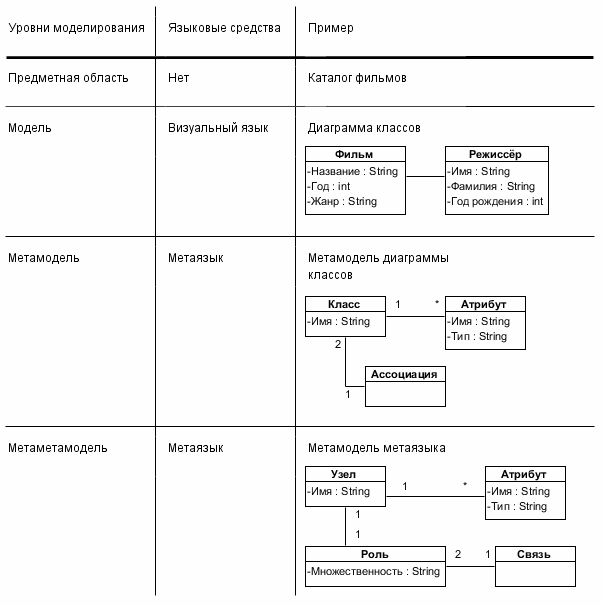
\includegraphics[width=0.7\textwidth]{metalevels.png}
	\end{center}
	\caption{Метауровни}
	\label{figure:metalevels}
\end{figure}

UML использует в своём стандарте строгую четырёхуровневую архитектуру метамоделирования. На нулевом уровне (M0) находятся объекты реального мира, которые надо моделировать, на первом уровне (M1) --- модель на визуальном языке, которая соответствует метамодели языка (уровня M2), которая, в свою очередь соответствует метаметамодели UML (уровня M3, в стандарте UML этот уровень занимает метаязык MOF). Так что, например, в метаметамодели определены понятия ``сущность'' и ``связь'', в метамодели диаграммы классов UML определены понятия ``класс'' и ``атрибут'' как экземпляры сущности ``сущность'' (обратите внимание, ``сущность'' сама является сущностью), между ними есть связь ``содержит'', являющаяся экземпляром связи ``связь''. В конкретной пользовательской модели определён класс ``Покупатель'', являющийся экземпляром сущности ``класс'', а пользовательские данные --- это конкретный покупатель, который является экземпляром класса ``Покупатель'' (см рисунок~\ref{figure:metalevelsExample}). Строгость архитектуры состоит в том, что сущности позволено быть экземпляром только одной сущности ровно на один метауровень выше (кроме сущностей метауровня M3, которые могут быть экземплярами лишь сущностей метауровня M3). Ограничение строгости существенно упрощает стандарт и его инструментальную поддержку.

\begin{figure}
	\begin{center}
		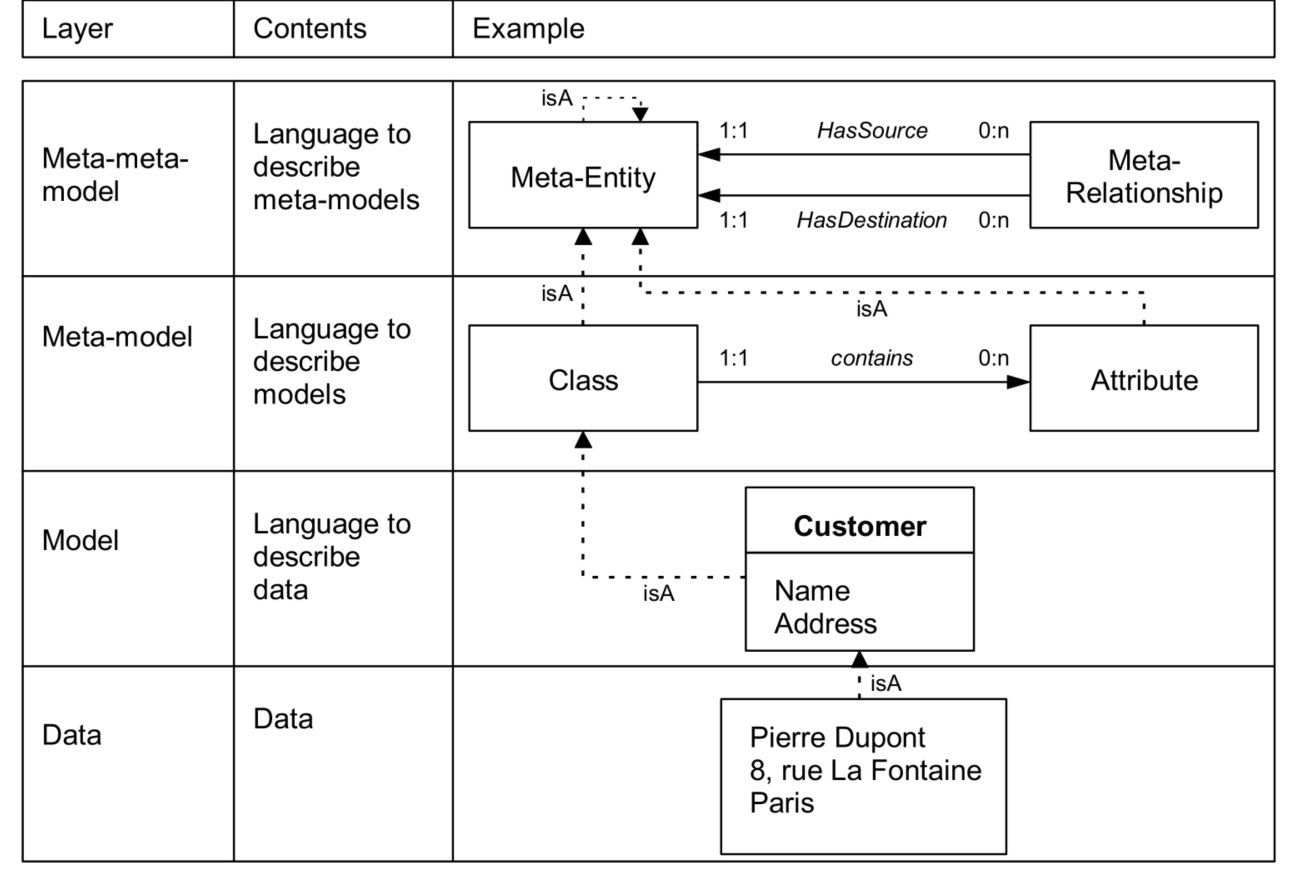
\includegraphics[width=0.6\textwidth]{bezivinExample.png}
	\end{center}
	\caption{Пример метауровней UML, из~\cite{bezivin1997ontology}}
	\label{figure:metalevelsExample}
\end{figure}

Отношение ``является экземпляром'' (и операция \textit{инстанцирования}, создающая экземпляр), пожалуй, самое важное в любой архитектуре, использующей метамоделирование, поскольку позволяет создавать элементы модели в соответствии с правилами, определяемыми метамоделью (что-то похожее на правила вывода в грамматике текстовых языков). Формально оно обычно не определяется, но интуитивно понимается как ``выдача'' конкретных значений атрибутам, определённым в типе. ``Является экземпляром'' близко наследованию, хотя бы потому, что отношение наследования определяется как отношение ``является'' и тоже заставляет связанные сущности иметь схожие свойства. Часто наследование и инстанцирование оказываются более-менее взаимозаменяемыми, иногда используются совместно (см., например, паттерн ``Powertype'' и работу~\cite{gonzalez2006powertype}). Важно обратить внимание, что инстанцирование и наследование всё-таки концептуально разные вещи --- например, наследование транзитивно, а инстанцирование --- нет.

\section{Проблемы строгого метамоделирования}

\subsection{Неоднозначность понятия ``Является экземпляром''}

Казалось бы, что всё просто и понятно, но уже в 1997 году появились работы, в которых указывалось, что что-то здесь не так (а UML только был стандартизован в 1997 году). Собственно, глубокое метамоделирование и другие подходы, о которых будет рассказано дальше, появились как попытка разрешить возникающие проблемы, но даже на сегодняшний день (UML 2.5.1) стандарт UML эти проблемы всё ещё имеет. Основная проблема состоит в том, что формально объект не является экземпляром класса. Сущность ``объект'' описана на метауровне M2 в метамодели диаграммы объектов, ``класс'' описан в метамодели диаграммы классов на уровне M2 же, так что из-за принципа строгости отношение ``является экземпляром'' не может их связывать. И, в общем-то, понятно, почему так --- на уровне M2 описываются элементы, которые требуется поддерживать в инструментах рисования диаграмм, метамодель --- это содержимое их палитры. Если бы объект был синтаксически экземпляром класса, то пришлось бы каждый раз, когда пользователь рисует на диаграмме класс, добавлять в палитру элемент ``объект этого класса'', от чего и авторы инструментов, и авторы диаграмм с ума бы сошли.

Из этой проблемы вытекает важное для реализации инструментов следствие --- пользователь может нарисовать диаграмму классов, нарисовать диаграмму объектов с объектами этих классов, но проверить, что все объекты действительно являются экземплярами правильных классов и имеют все нужные атрибуты правильных типов чисто синтаксически невозможно, то есть стандарт UML оставляет это на откуп авторам инструментов. Первый предложенный способ борьбы с этой проблемой~\cite{bezivin1997ontology} --- это чётко разделять ``лингвистическое'' отношение ``явялется экземпляром'' и ``онтологическое'' отношение, первое интересно инструментам, второе --- пользователям, при этом второе водится на уровне M2 (метамодели языка), а первое --- на уровне M3 (метаметамодели), и они никак друг с другом не связаны. В современном UML есть только лингвистические отношения, поэтому приходится очень внимательно объяснять студентам, что хоть объект и экземпляр класса, но не в том же самом смысле, что класс является экзампляром метакласса. Суть поясняет рисунок~\ref{figure:isAExample}.

\begin{figure}
	\begin{center}
		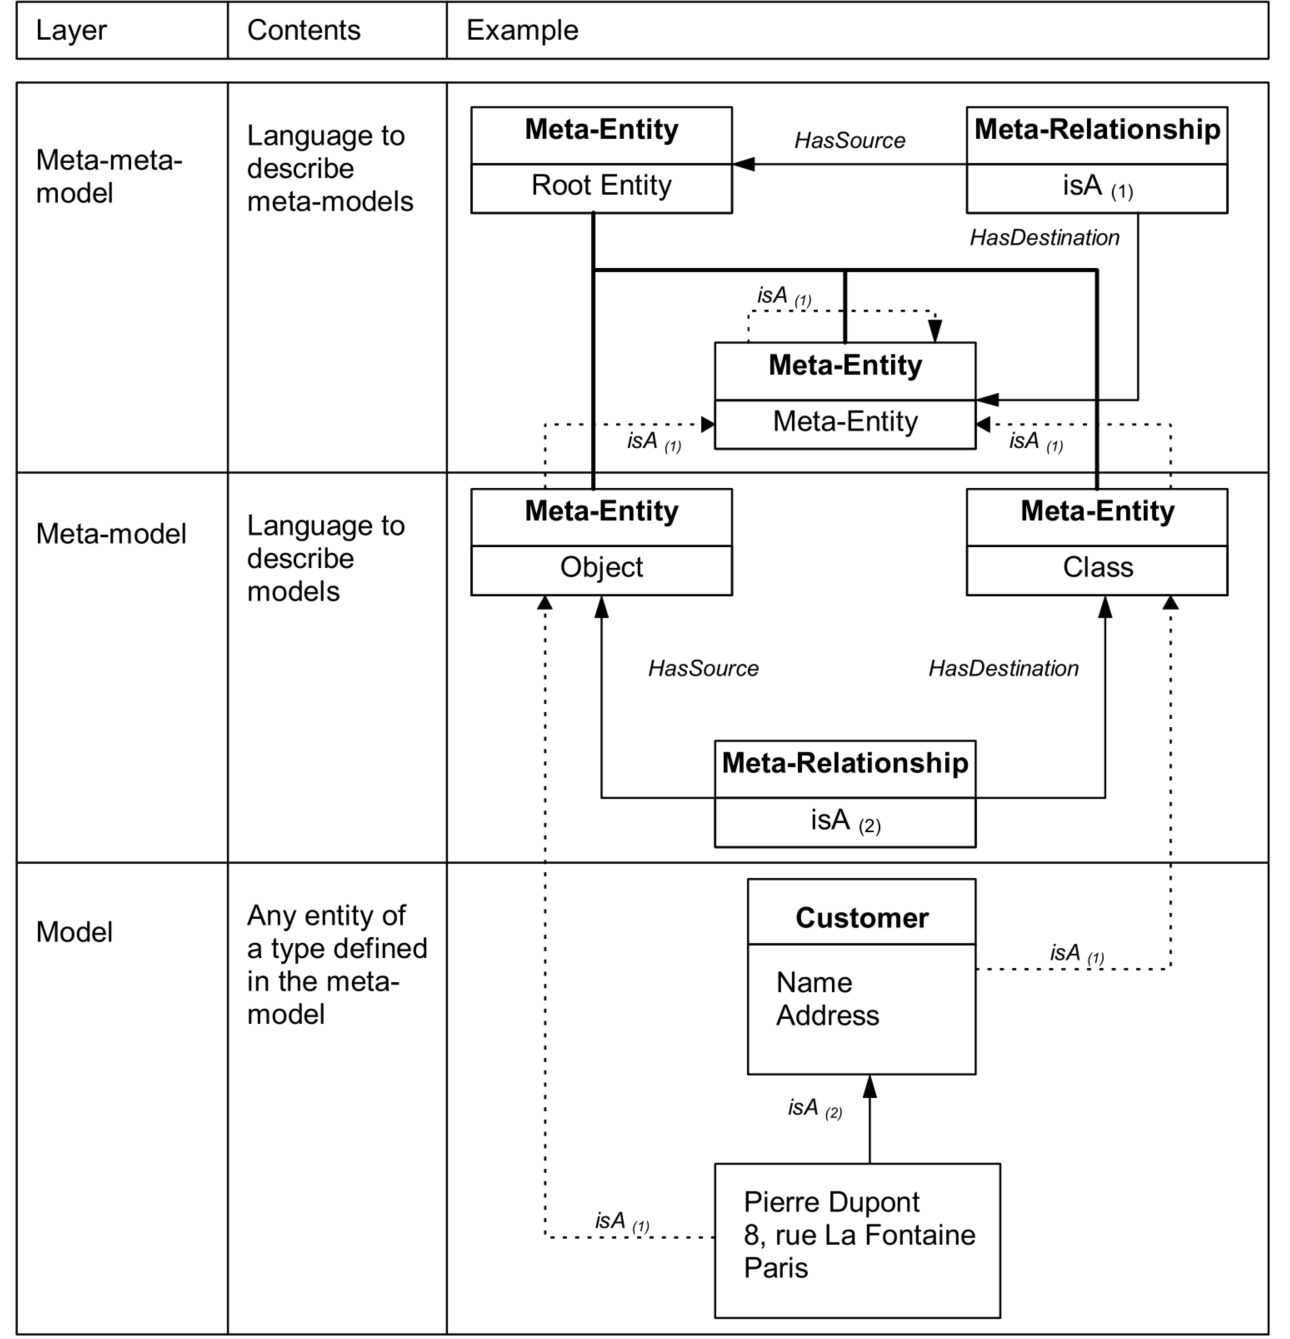
\includegraphics[width=0.6\textwidth]{bezivinIsA.png}
	\end{center}
	\caption{Лингвистическое и онтологическое отношения ``является экземпляром'', из~\cite{bezivin1997ontology}}
	\label{figure:isAExample}
\end{figure}

Более подробно та же проблема обсуждается в работе~\cite{atkinson2001multilevel}, рисунок~\ref{figure:atkinsonInstanceOf} взят оттуда и иллюстрирует проблему ещё лучше. Тут в метамодели описано, что компонент может содержать в себе узлы (это реальный пример куска метамодели диаграммы компонентов UML), в модели конкретной системы описан конкретный компонент C и конкретный узел N, и в модели состояния работающей системы есть конкретный экземпляр компонента C, связанный с конкретным экземпляром узла N, но формально они никак со своими типами не связаны.

\begin{figure}
	\begin{center}
		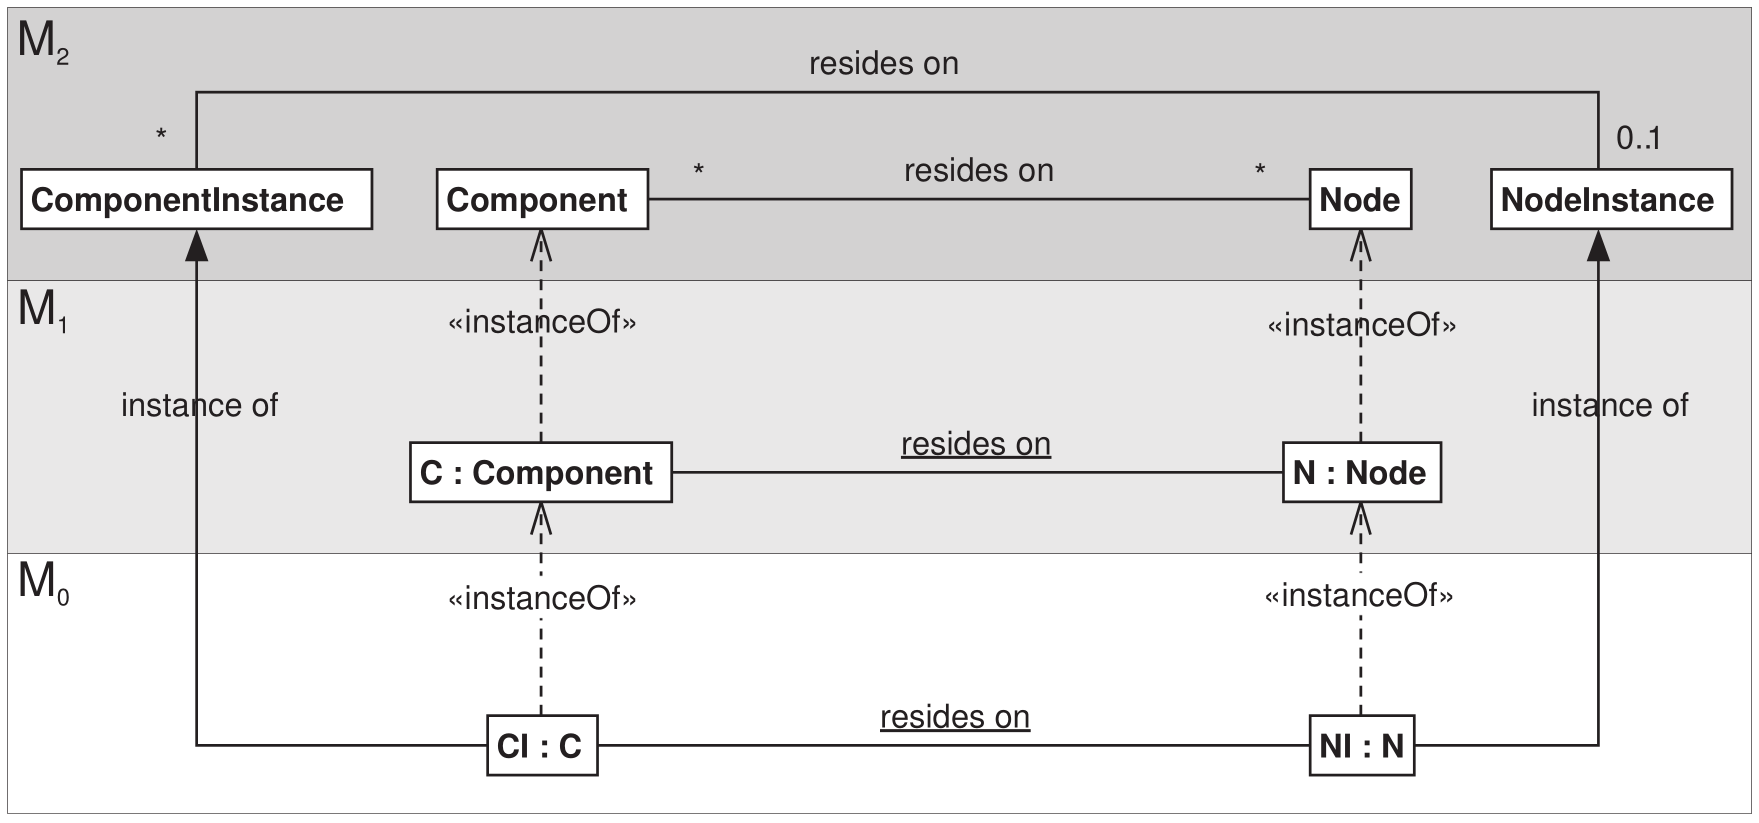
\includegraphics[width=0.7\textwidth]{atkinsonInstanceOf.png}
	\end{center}
	\caption{Ещё один пример неоднозначности ``является экземпляром'', из~\cite{atkinson2001multilevel}}
	\label{figure:atkinsonInstanceOf}
\end{figure}

\subsection{Умножение сущностей}

В принципе, неоднозначность ``instanceOf'' с прагматической точки зрения не так страшна, в конце концов в текстовых языках тоже контроль типов выполняется отдельной фазой компиляции и никогда не выносится в грамматику. В UML есть текстовый подъязык задания семантических ограничений OCL, который в целом может решить проблему, так что люди живут с этим. Более важная с практической точки зрения проблема состоит в том, что на каждом метауровне нам требуется заново объявлять понятия типов и экземпляров, если мы хотим язык с типизацией, и симулировать ``семантическое'' создание экземпляра через синтаксическое отношение ``является экземпляром'' и пару сущностей, соответствующих понятиям ``тип'' и ``экземпляр типа'' в метамодели. В самой метамодели UML это не страшно, но вспомним, что и у метамодели есть метамодель, и там тоже нужны понятия ``тип'' и ``экземпляр'', по сути те же самые, но формально другие (и никак не связанные с уже введёнными). Рисунок~\ref{figure:atkinsonDuplication} иллюстрирует проблему на простом примере с собакой Фидо, которая собака, но вместе с тем ``экземпляр'', тогда как ``собака'' сама по себе экземпляр класса ``класс'', поэтому может рассматриваться как экземпляр сущности ``экземпляр'' из метаметамодели.

\begin{figure}
	\begin{center}
		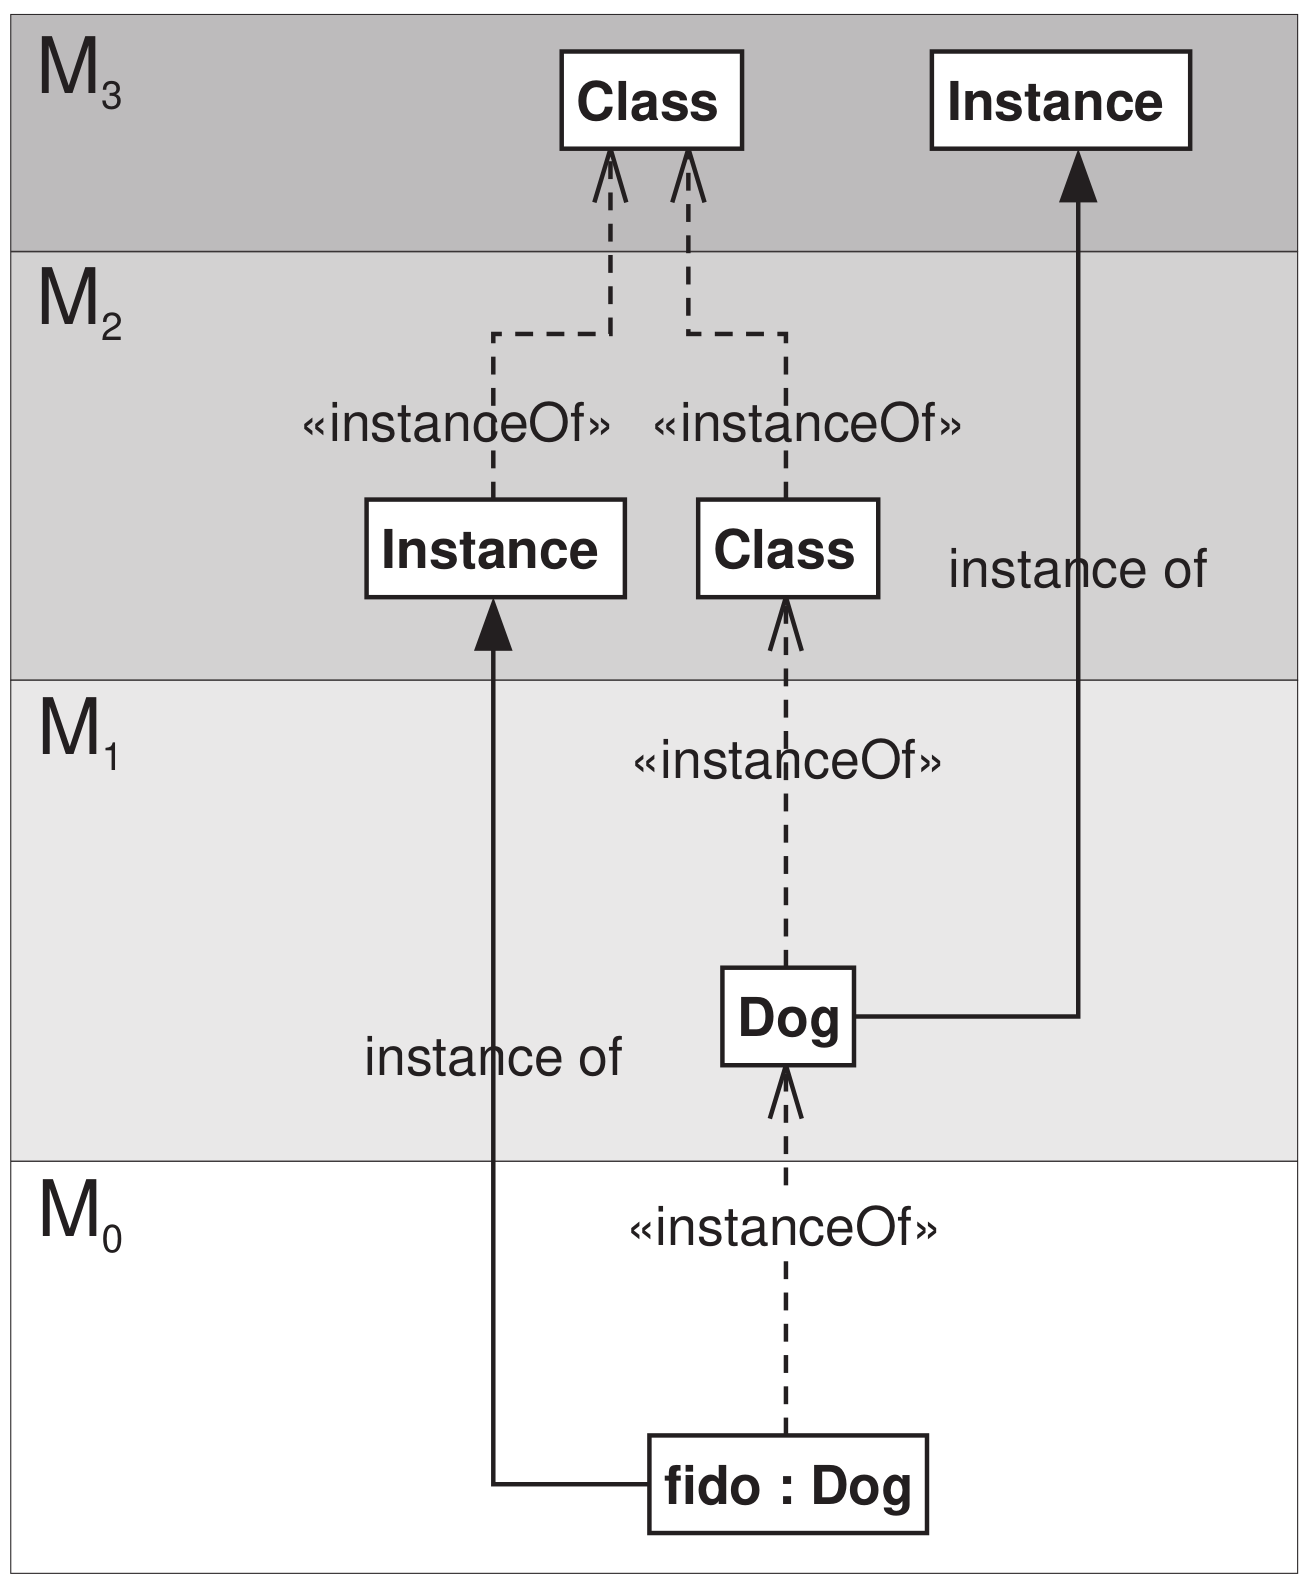
\includegraphics[width=0.4\textwidth]{atkinsonDuplication.png}
	\end{center}
	\caption{Умножение понятий ``класс'' и ``экземпляр'', из~\cite{atkinson2001multilevel}}
	\label{figure:atkinsonDuplication}
\end{figure}

Это плохо концептуально, тем, что лингвистические отношения ``является экземпляром'' связывают сущности на два метауровня выше, и чисто практически, метамодели не по делу растут. В стандарте UML используются некоторые словесные ухищрения, чтобы не писать по два раза одно и то же (в духе ``вот тут мы вводим новый класс Classifier, который получен копированием из такого же в MOF, но он новый''), и то некоторые понятия там вводятся несколько раз на разных метауровнях, что делает метамодель трудной для понимания. Ещё одна важная проблема состоит в том, что вводим понятия ``тип'' и ``экземпляр'' мы не просто так, а чтобы определить понятие ``является экземпляром'' (онтологическое), и, поскольку мы это делаем на каждом метауровне заново, могут вкрасться неконсистентности и ошибки, да и реализовать в инструментах это сложно.

\subsection{Подпрограммы в TRIK Studio}

Ещё одна проблема с классической четырёхуровневой схемой в том, что иногда четырёх уровней просто недостаточно. Чисто практическая задача, с которой мы сами столкнулись --- это реализация подпрограмм в среде TRIK Studio. Если учить детей программированию, то надо учить их сразу избегать монолитных программ, а придерживаться принципа декомпозиции, решая каждую подзадачу отдельно и объединяя их в основной программе. Поэтому в TRIK Studio необходимо было реализовать поддержку подпрограмм, и, поскольку TRIK Studio (а точнее, среда QReal, на которой она основана) придерживается классической четырёхуровневой архитектуры метамоделирования, реализация подпрограмм доставила нам много проблем. 

Что хотелось (и что в итоге было сделано, но ценой переработки где-то трети кода ядра системы): иметь в визуальном языке элемент ``Подпрограмма'', который при вытаскивании его на сцену (\textit{инстанцировании}) порождал бы новую диаграмму в проекте --- с ``кодом'' подпрограммы, порождал бы на основной диаграмме узел ``экземпляр подпрограммы'' и добавлял бы этот узел ещё и в пользовательскую палитру, так, чтобы его самого можно было вытащить на сцену и вызвать ту же подпрограмму ещё раз. Кроме того, мы хотели, чтобы у каждой подпрограммы был свой набор параметров и даже своя картинка (иначе их сложно было визуально отличить друг от друга). Как это выглядит в работающей системе показано на рисунке~\ref{figure:trikStudio}. Архитектура метауровней в реализации нам никак не помогла, весь код для поддержки подпрограмм был написан вручную, и с каждым узлом ``экземпляр подпрограммы'' была связана структура данных, описывающая его дополнительные свойства (так называемые \textit{динамические свойства}), поддержка которых была реализована в редакторе. Концептуально динамические свойства занимали промежуточное положение между моделью и метамоделью.

\begin{figure}
	\begin{center}
		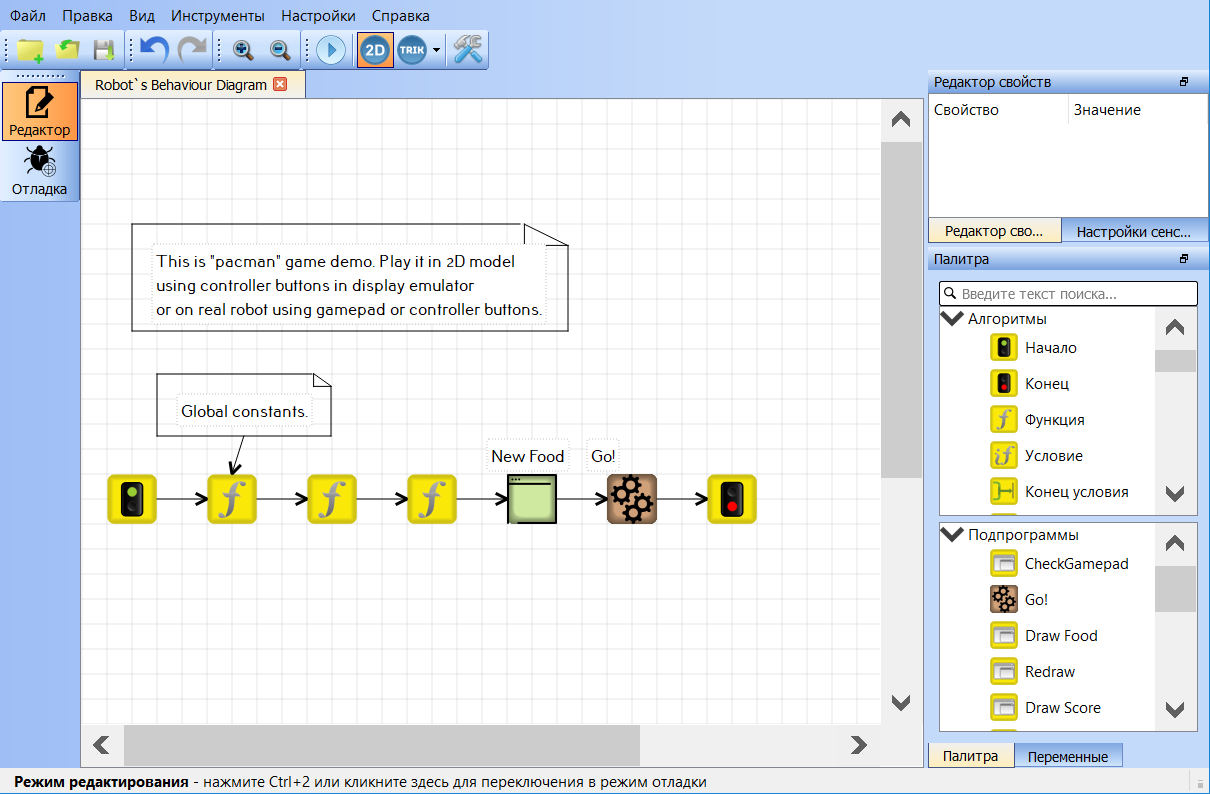
\includegraphics[width=\textwidth]{trikStudio.png}
	\end{center}
	\caption{Окно среды TRIK Studio с экземпляром подпрограммы}
	\label{figure:trikStudio}
\end{figure}

\section{Глубокое метамоделирование}

Решения вышеизложенных проблем начали активно предлагаться в начале 2000-х, когда началась разработка стандарта UML 2.0. В те времена вышло сразу несколько статей, которые предлагали свои подходы к метамоделированию, вплоть до ``выкинуть весь существующий стандарт и использовать именно наш метаязык'' (см., например,~\cite{alvarez2001mml}). В 2005 году стандарт UML 2.0 наконец вышел, внесённые предложения были проигнорированы и каких-то радикальных изменений не произошло, UML использует строгую четырёхуровневую архитектуру до сих пор. Однако некоторые идеи того времени заслуживают обсуждения просто потому, что либо нашли своё применение, либо могут быть применены при разработке предметно-ориентированных языков и инструментов, которые их поддерживают. Одна из первых таких идей --- это ``глубокое метамоделирование'', предложенное Колином Аткинсоном и Томасом Кюне в 2001 (идеи, как обычно, витали в воздухе с 1997, но, пожалуй, самая известная работа по этой теме датирована именно 2001 годом).

Идея ``глубокого метамоделирования'' состоит в том, что отношение ``является экземпляром'' может оказывать влияние не только на один метауровень вниз, как в классической схеме, но и на метауровни ниже, заставляя тем самым экземпляры экземпляров метатипа иметь определённые свойства. Простой пример (из работы~\cite{gonzalez2006powertype}): при моделировании методологии разработки ПО (в стиле SEMAT или SPEM) хочется описать метакласс ``Вид задачи'', у которого есть поля ``Имя'', ``Важность'' и т.д., от него порождать классы-задачи (например, ``Писать код'' или ``Разрабатывать архитектуру''), у каждого из которых должен быть атрибут ``Кто отвечает'', ``Текущий статус'' и т.д., чтобы от них можно было порождать экземпляры задач (например, ``Вася должен реализовать класс Controller'') и заполнять эти поля. Естественно, хотелось бы описывать эти поля ещё на метауровне, прописав их в ``Вид задачи'', но для классов-задач эти поля ещё не должны принимать значения, а должны передаваться их экземплярам.

Реализовать это можно, если рассматривать каждую сущность не как класс или экземпляр, а как сущность, которая может иметь одновременно и свойства класса, и свойства экземпляра, то есть и хранить в себе данные, и представлять собой схему для создания объектов, хранящих в себе данные, соответствующие этой схеме. В глубоком метамоделировании это достигается добавлением каждому элементу модели свойства \textit{potency} --- целого числа, показывающего, на сколько метауровней вниз этот элемент может быть инстанцирован --- и свойства \textit{level} --- целого числа, показывающего номер метауровня, на котором находится элемент (при этом, как и в UML, нулевой уровень --- это уровень пользовательских данных, самый большой метауровень соответствует метамета...модели). Операция инстанцирования применима только к элементам с положительным значением potency и уменьшает potency и level на 1. Обычный класс в UML имеет potency 1 и level 1, абстрактный класс --- potency 0 и level 1, желаемый нами метакласс ``Вид задачи'' имел бы potency 2.

Эти свойства применимы ко всем элементам модели, в том числе, к атрибутам, что приводит к возможности введения понятия \textit{dual fields} --- полей, которые имеют значение И могут быть инстанцированы, возможно, с переопределением их значения. В противоположность им \textit{single field} приобретает значение только когда его potency принимает значение 0. Dual field с potency n можно понимать как множество из n single field-ов, где единственное поле с potency 0 имеет своё значение и при инстанцировании выкидывается из множества, при этом potency всех остальных полей уменьшаются на единицу и одно из них получает значение.

Если попробовать перерисовать с использованием глубокого метамоделирования рисунок~\ref{figure:atkinsonInstanceOf}, то получится модель, изображённая на рисунке~\ref{figure:deepComponents}. У каждого элемента модели числом рядом с ним указана его potency, подчёркнутые атрибуты --- single fields, неподчёркнутые --- dual fields. Важно, что поскольку отношения тоже имеют potency, отношение ``resides on'', которое в метамодели из~\ref{figure:atkinsonInstanceOf} (и из стандарта UML тоже) было дублировано и имело проблемы с проверкой синтаксической корректности, здесь естественным образом инстанцируется дважды и корректность модели на уровне M0 обеспечивается уже не семантическими ограничениями, а просто определением глубокого инстанцирования.

\begin{figure}
	\begin{center}
		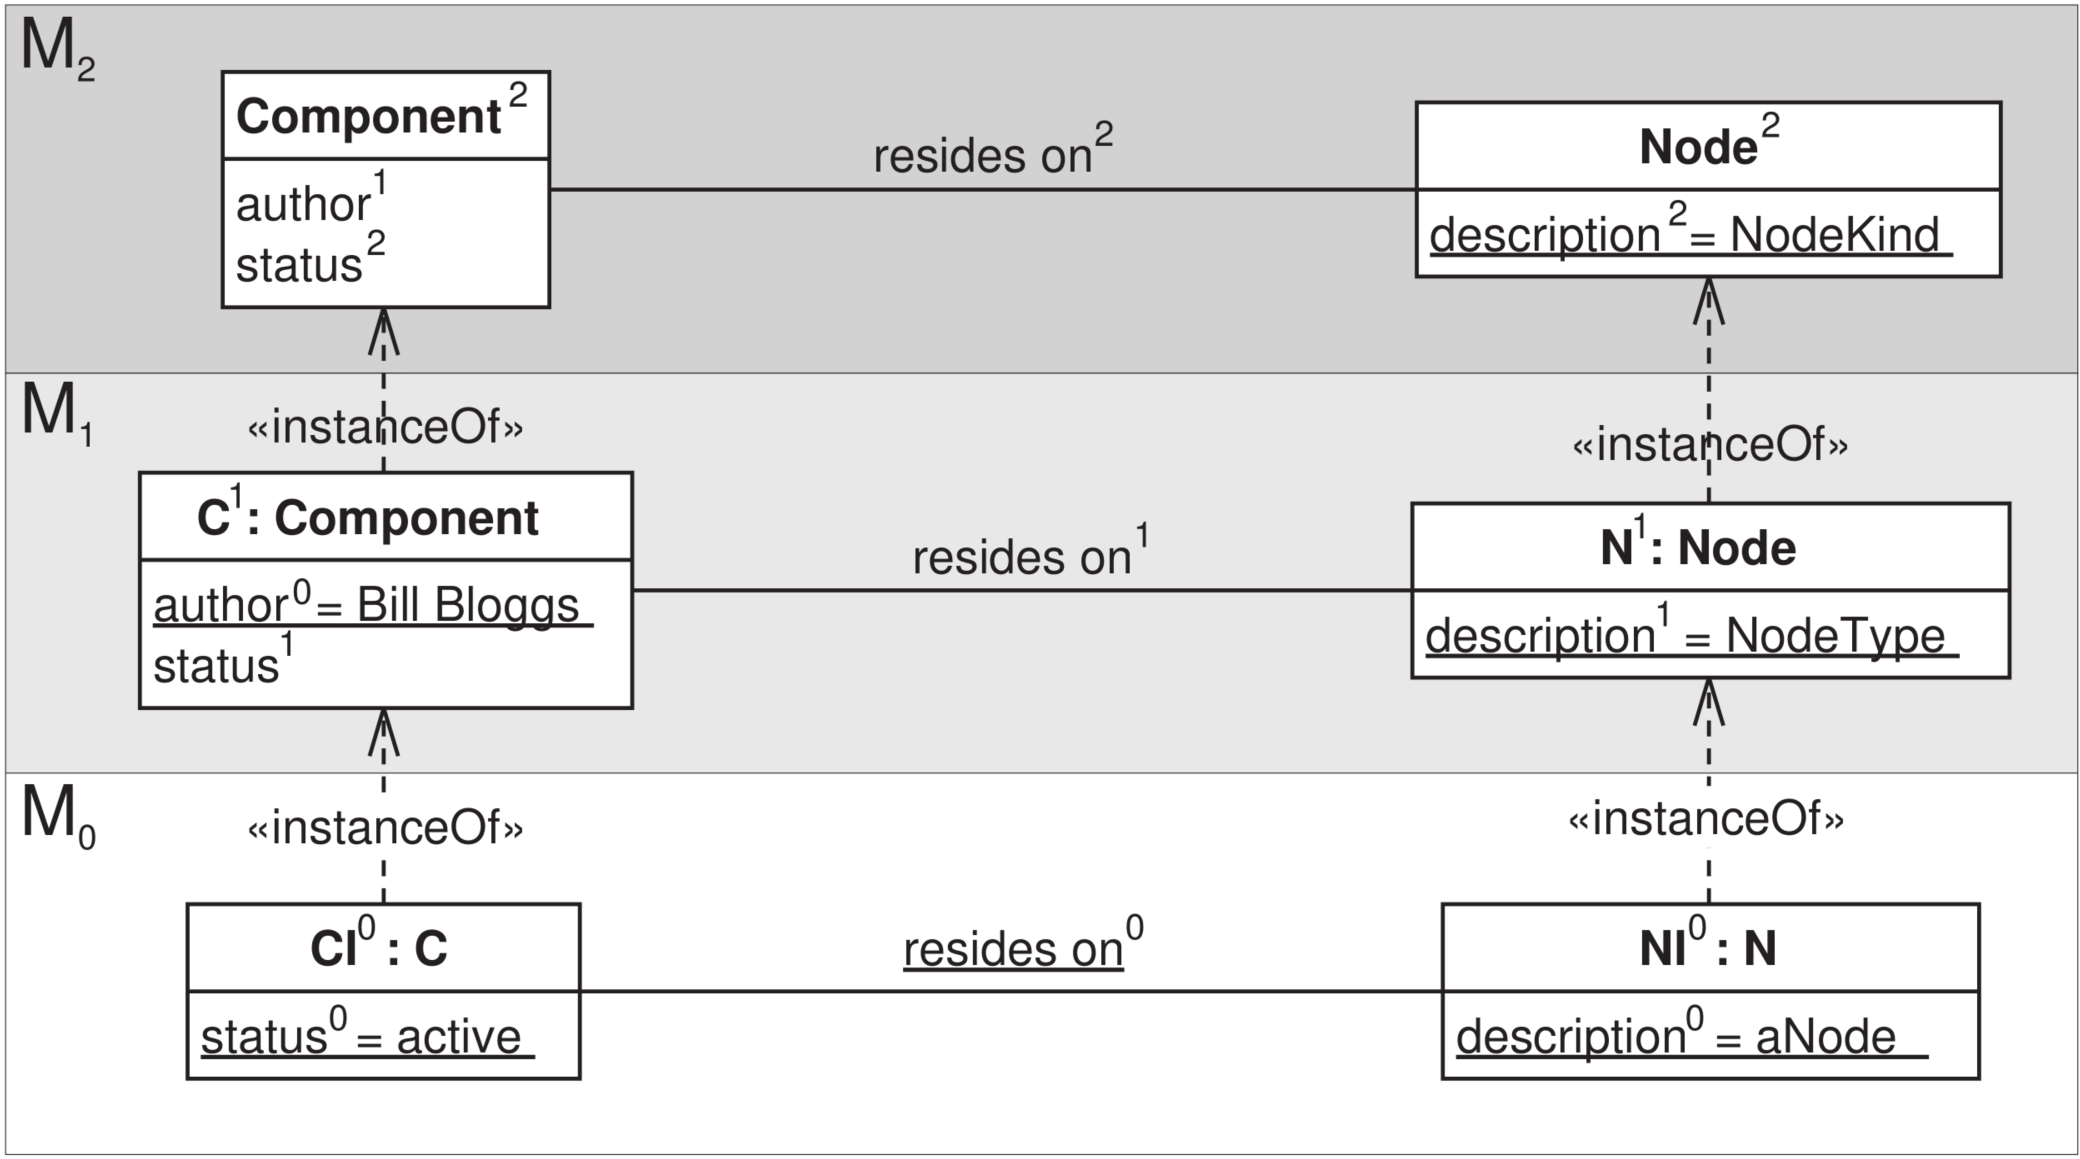
\includegraphics[width=0.7\textwidth]{deepComponents.png}
	\end{center}
	\caption{Метамодель диаграммы компонентов, использующая глубокое метамоделирование, из~\cite{atkinson2001multilevel}}
	\label{figure:deepComponents}
\end{figure}

Работа~\cite{atkinson2001multilevel} завершается предложением минимальной рефлексивной (то есть являющейся экземпляром самой себя) метаметамодели, которая поддерживает глубокое метамоделирование, она представлена на рис.~\ref{figure:momm}. Авторы сами говорят, что метаметамодели весьма примерна и служит скорее для иллюстрации концепций (и это правда, например, судя по модели, у них атрибут не может иметь значения). 

\begin{figure}
	\begin{center}
		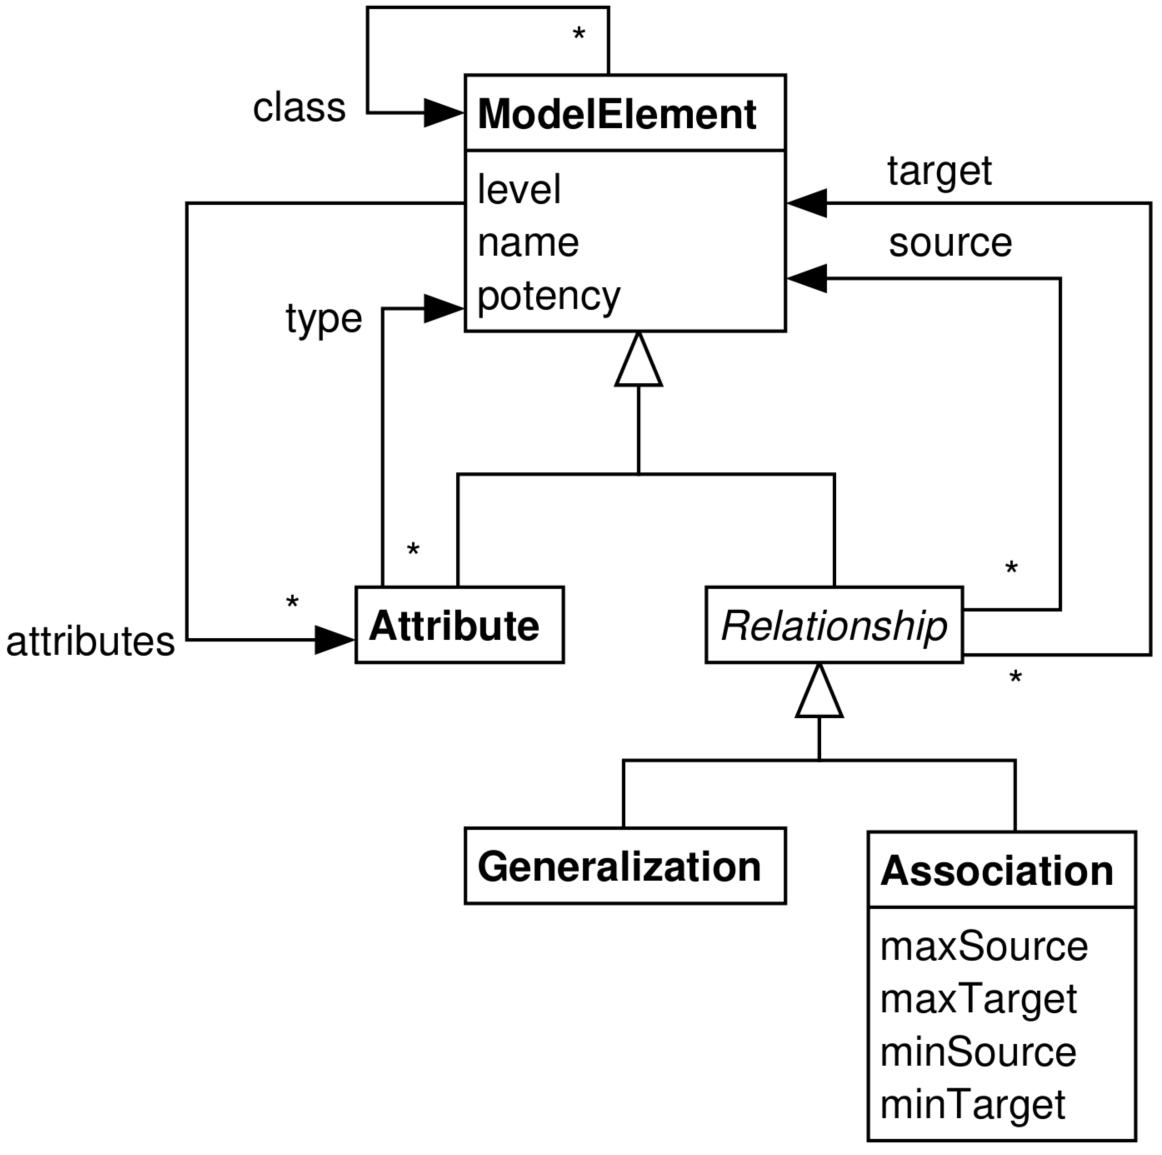
\includegraphics[width=0.5\textwidth]{momm.png}
	\end{center}
	\caption{Метаметамодель для глубокого метамоделирования, из~\cite{atkinson2001multilevel}}
	\label{figure:momm}
\end{figure}

\section{Ортогональное метамоделирование}

Дальнейшим развитием идей~\cite{atkinson2001multilevel} стала даже более популярная работа~\cite{atkinson2003model} (более тысячи цитирований по данным Google Scholar). Если с дублированием концепций глубокое метамоделирование нам помогает, то неоднозначность понятия ``является экземпляром'' всё ещё существует, и наивная попытка реализовать глубокое метамоделирование в инструменте натолкнётся на это очень быстро --- ``Вася реализует класс Controller'' является экземпляром класса ``Писать код'', который является экземпляром класса ``Тип задачи'', да, но отношение ``Является экземпляром'' нетранзитивно, так что ``Вася реализует класс Controller'' не является экземпляром класса ``Тип задачи''. Как инструмент ``догадается'', как рисовать конкретную задачу, какие действия с ней позволены пользователю, как сохранять на диск информацию о ней и т.д.? Мы, наверное, не хотим в модель методологии (где определяется задача ``Писать код'') вносить ещё и определение служебной информации или ``протаскивать'' её как dual fields с уровня метамодели (определяя их в классе ``Тип задачи''). Не хотим, например, потому, что инструмент должен как-то ``догадаться'', что эти поля служебные и не должны показываться пользователю в редакторе свойств, а должны правильно интерпретироваться самим редактором.

Всё это наводит нас на мысль, что модель уровня M0 в глубоком метамоделировании на самом деле является не только экземпляром своей ``семантической'' метамодели M1 (возможно, определяемой пользователем), но и метамодели, определяемой реализацией редактора --- например, что у каждой сущности на диаграмме должно быть поле, где написано, узел это или ребро графа модели, и если узел, то у него должно быть свойство, где написано, как должен этот узел выглядеть на диаграмме, можно ли его растягивать и кидать внутрь элементы. Таким образом, можно различать ``лингвистическое'' инстанцирование, которое каждую сущность модели делает экземпляром некоторой сущности визуального языка, и ``онтологическое'' инстанцирование, где каждая сущность --- это экземпляр ``онтологической'' метамодели, содержащей ``идеи'' сущностей. В отличие от предложения из~\cite{bezivin1997ontology}, где онтологическое инстанцирование объявлялось просто отношением, определяемым в лингвистической метамодели и ему запрещалось давать какой-то специальный смысл, Аткинсон с Кюне предлагают рассматривать эти отношения как равноправные и просто смотреть на одну и ту же модель с разных точек зрения. Инструментальным средствам более интересна лингвистическая точка зрения, пользователю --- онтологическая, а поскольку они существуют в рамках единой инфраструктуры, легко обеспечить их соответствие. Смысл происходящего поясняют рисунки~\ref{figure:linguisticView} и~\ref{figure:ontologicalView}.

\begin{figure}
	\begin{center}
		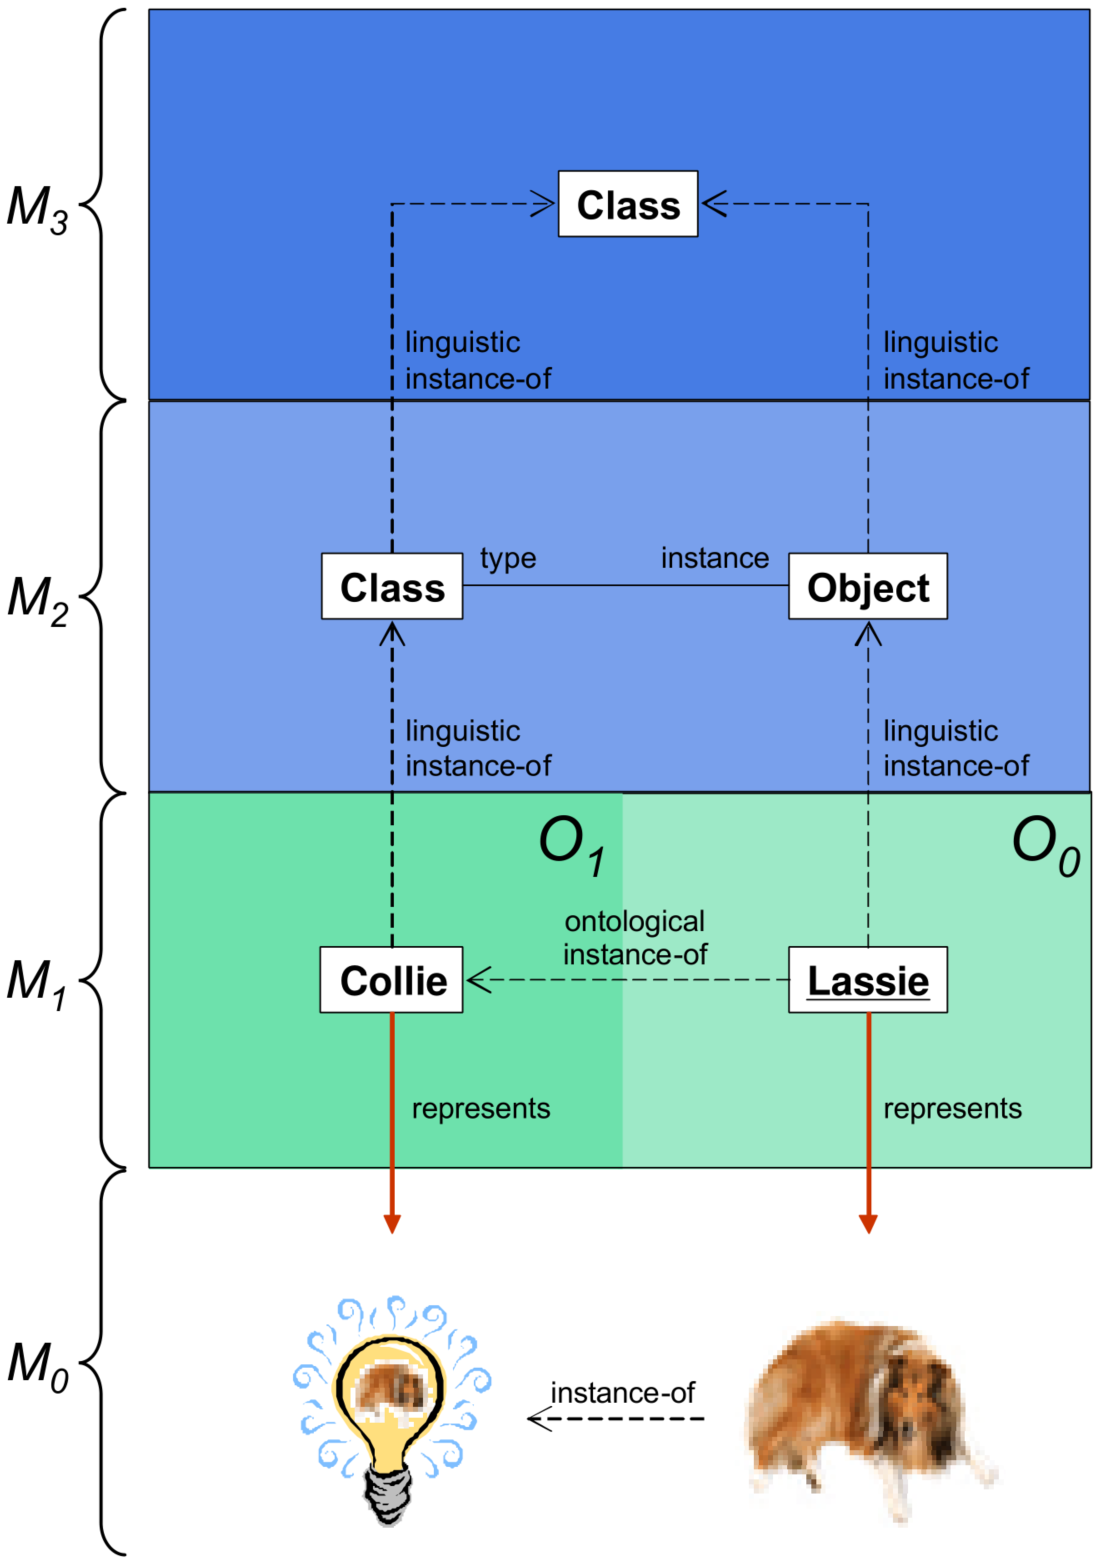
\includegraphics[width=0.4\textwidth]{linguisticView.png}
	\end{center}
	\caption{Лингвистическая точка зрения на модель, из~\cite{atkinson2003model}}
	\label{figure:linguisticView}
\end{figure}

\begin{figure}
	\begin{center}
		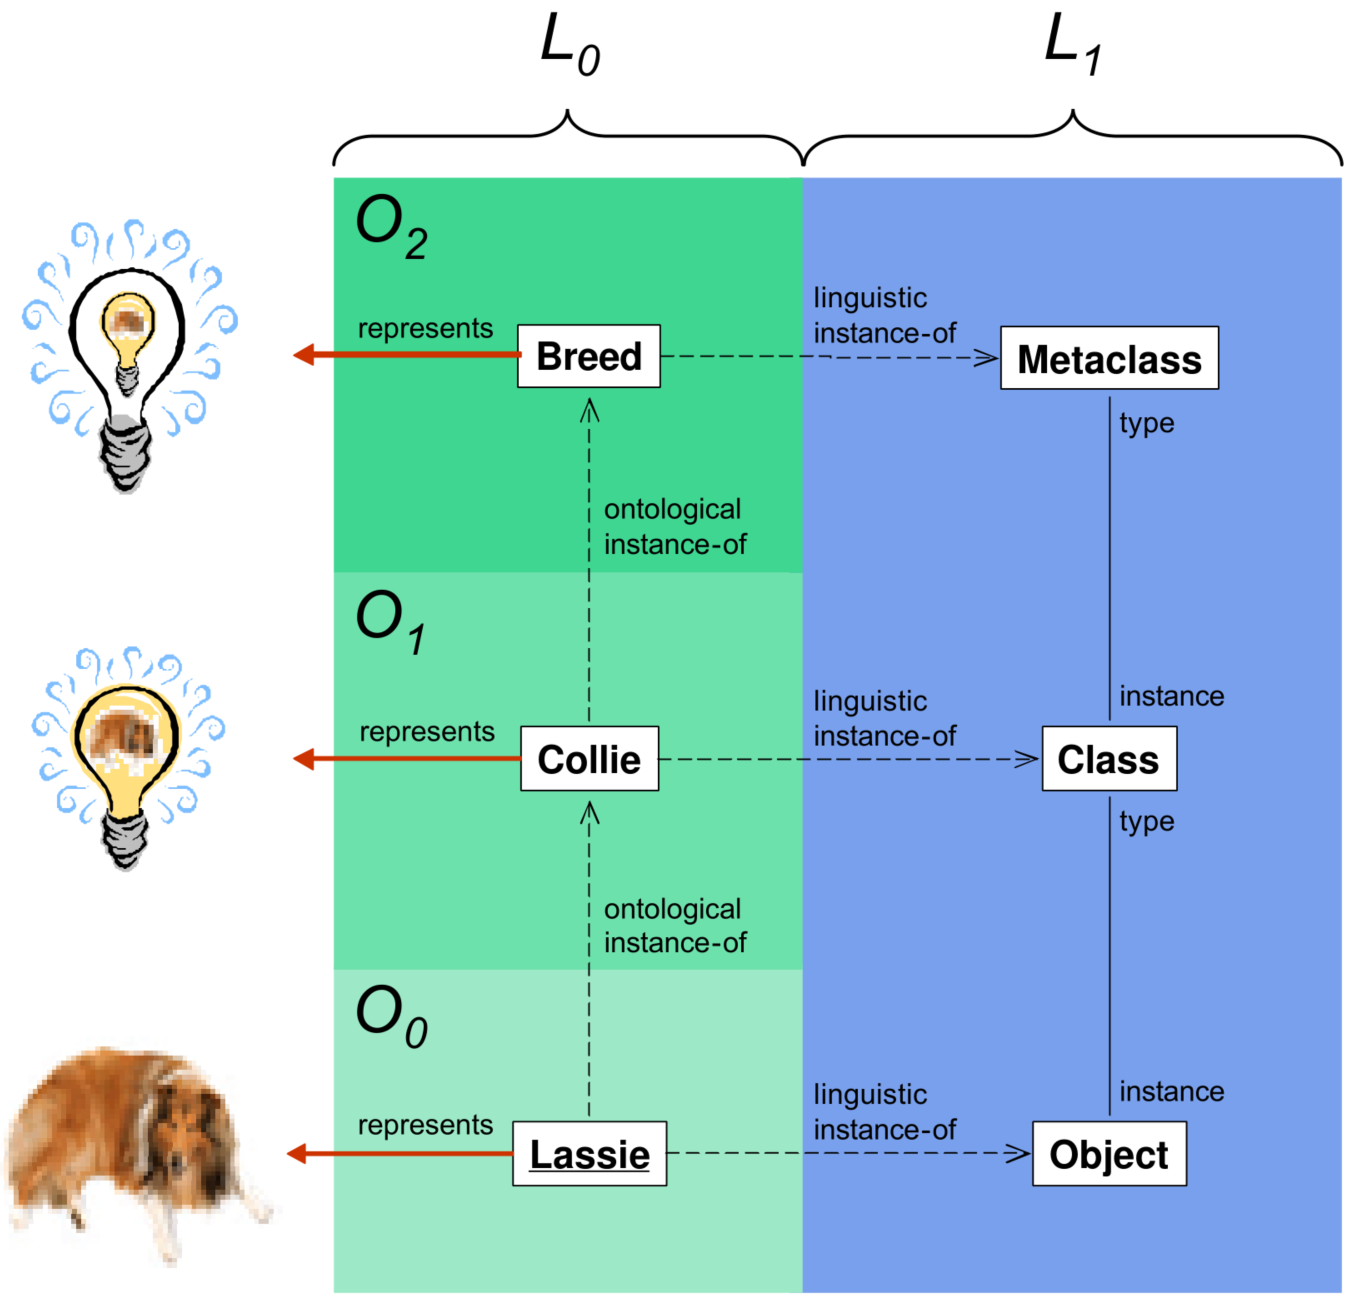
\includegraphics[width=0.5\textwidth]{ontologicalView.png}
	\end{center}
	\caption{Онтологическая точка зрения на модель, из~\cite{atkinson2003model}}
	\label{figure:ontologicalView}
\end{figure}

Такой подход хорошо согласуется с существующими архитектурами метамоделирования (если стереть границы онтологических метауровней, получится в точности классическая строгая четырёхуровневая схема), хорошо работает с глубоким метамоделированием (каждый вид инстанцирования может быть глубоким), и даже хорошо работает с существующими в реальной жизни моделями, например, биологической классификацией живых существ, изображённой на рисунке~\ref{figure:biologicalClassification}. Единственная проблема такой схемы --- сложность (как концептуальная, так и сложность реализации). Некоторый, правда, весьма слабый аналог онтологической классификации появился и в UML 2.0 --- механизм профилей. Профиль позволяет задать для существующих классов метамодели UML пользовательские свойства, тем самым фактически описав онтологическую метамодель для моделей, соответствующих профилю.

\begin{figure}
	\begin{center}
		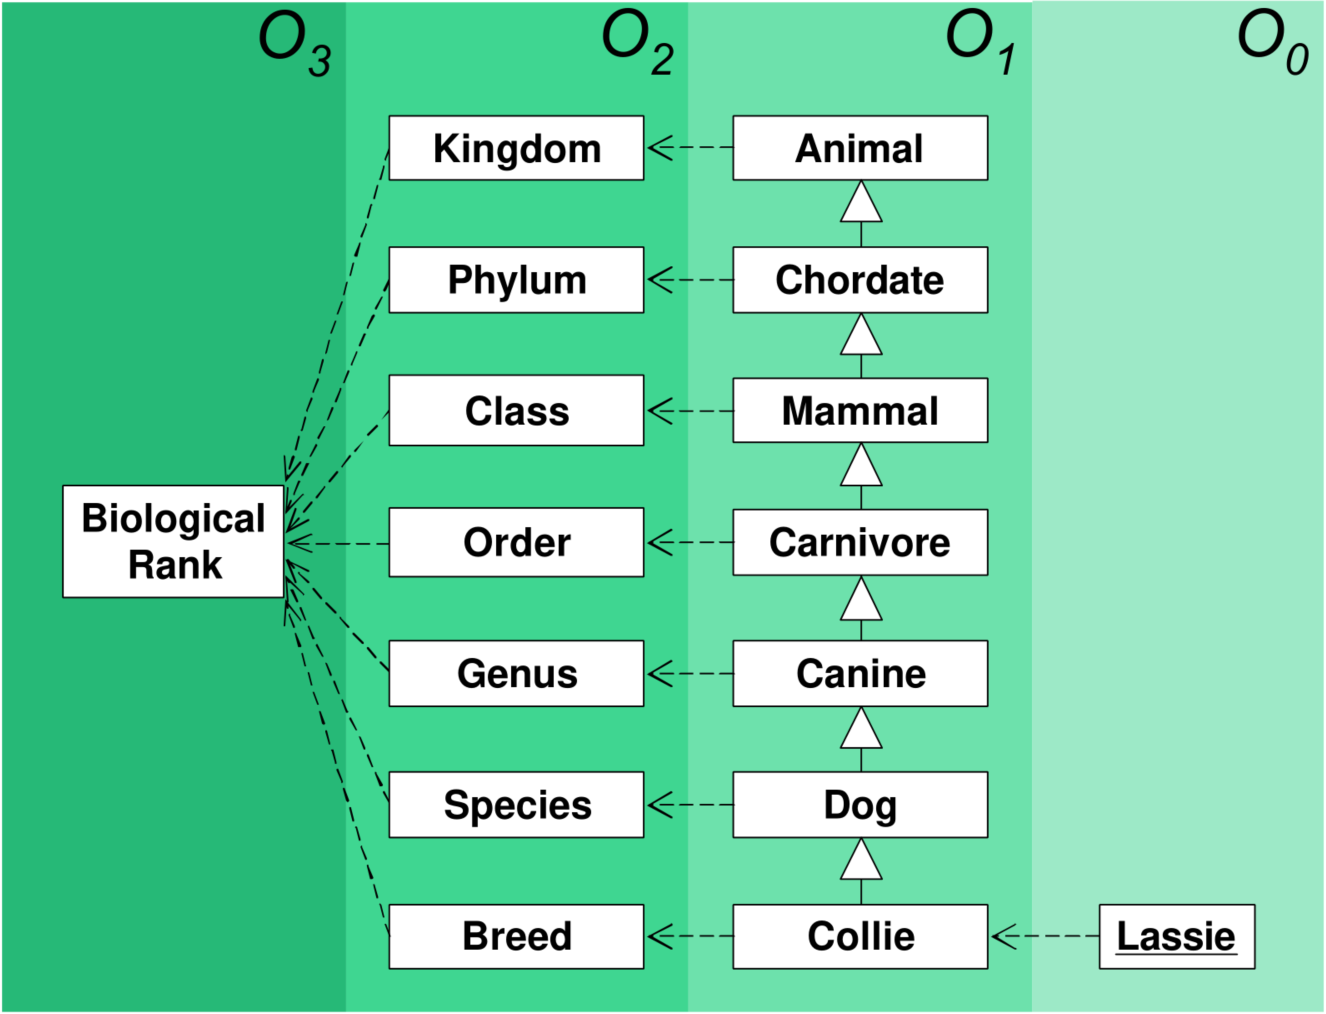
\includegraphics[width=0.5\textwidth]{biologicalClassification.png}
	\end{center}
	\caption{Онтологическая точка зрения на биологическую классификацию, из~\cite{atkinson2003model}}
	\label{figure:biologicalClassification}
\end{figure}

\section{Существующие реализации}

\subsection{Melanee}

Инструменты визуального моделирования, которые используют принципы глубокого метамоделирования, начали появляться относительно недавно, один из первых --- разработка под руководством самого Аткинсона, Melanee\footnote{Melanee home page, URL: \url{http://www.melanee.org} (дата обращения: 05.02.2018)}~\cite{atkinson2016melanee}, примерно 2012 года. Это инструмент, реализованный на Eclipse Modeling Framework, поддерживающий одновременно графические, текстовые и даже табличные нотации. Лингвистическая метаметамодель там фиксирована, из неё пользователю предлагается сделать метамодель (возможно, использующую несколько онтологических уровней: ``компания'' -> ``IT-компания'' -> ``Терком''), и по этой метамодели рисовать модели уже на конкретном языке (непонятно, правда, зачем). Выглядит инструмент так, как показано на рисунке~\ref{figure:melanee}.

\begin{figure}
	\begin{center}
		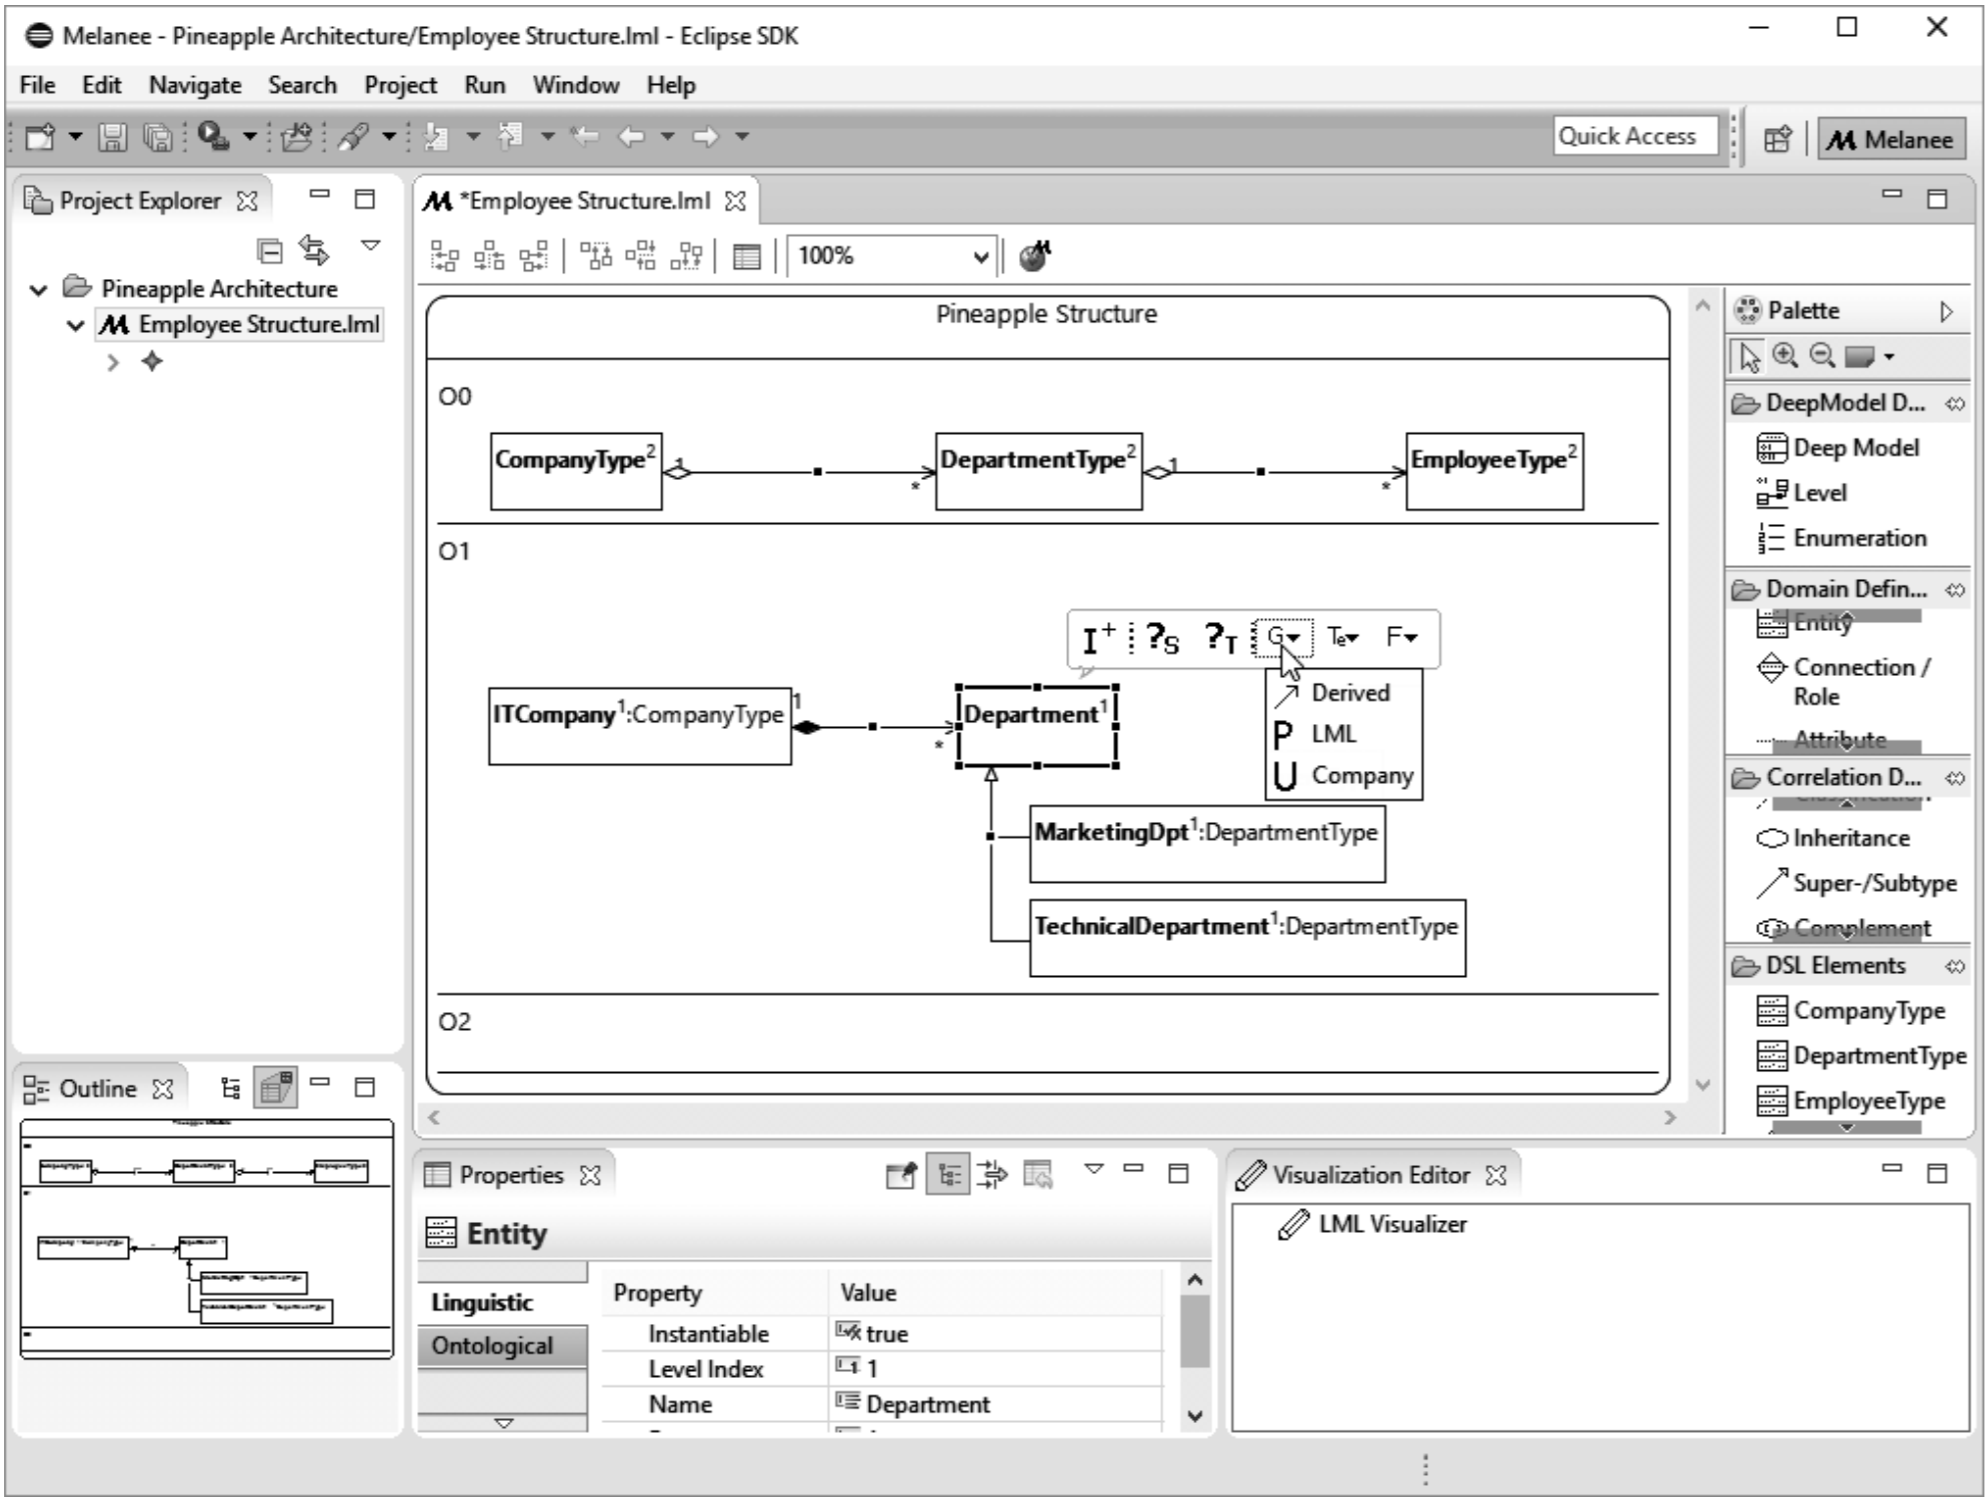
\includegraphics[width=0.8\textwidth]{melanee.png}
	\end{center}
	\caption{Пользовательский интерфейс системы Melanee, из~\cite{atkinson2016melanee}}
	\label{figure:melanee}
\end{figure}

\subsection{MetaDepth}

Даже более старая работа по этому поводу --- система MetaDepth\footnote{MetaDepth home page, URL: \url{http://metadepth.org/} (дата обращения: 05.02.2018)}~\cite{de2010deep}, от авторов $AToM^3$ J. De Lara и E. Guerra. Интересна тем, что она текстовая, никаких визуальных редакторов по метамоделям не генерируется, но умеет работать с Epsilon (это такой набор библиотек для Eclipse), поэтому умеет генерировать код по (текстовым) моделям, выполнять разные преобразования моделей (в том числе рефакторинги) и т.д. Пожалуй, первая известная реализация идей Аткинсона в коде.

\subsection{WebDPF}

Более свежая система --- WebDPF\footnote{WebDPF home page, URL: \url{http://dpf.hib.no/} (дата обращения: 05.02.2018)}~\cite{rabbi2016webdpf}, это уже браузерный инструмент (где-то 2016 года), имеющий в основе глубокое метамоделирование, но умеющий ещё много чего. Прежде всего, команда из университета Бергена занимается ограничениями на модели, так что WebDPF имеет интересную систему описания ограничений, чем-то похожую на контекстные ограничения из диссертации Александра Иванова --- ограничения описываются как отношения на графе метамодели. Что интересно, что по ограничениям строятся правила автодополнения --- редактор умеет предлагать элементы, которые надо нарисовать следующими, чтобы модель начала удовлетворять ограничениям. Кроме того, модель и метамодель рисуются на одной сцене, и можно попросить тул визуализировать отношения ``является экземпляром''. При этом у метамодели может быть своя метамодель и т.д. вверх по метауровням. Скриншот инструмента представлен на рисунке~\ref{figure:webdpf}, но вообще инструмент до сих пор работает на сайте университета, и поскольку он браузерный, на него можно без проблем посмотреть вживую.

\begin{figure}
	\begin{center}
		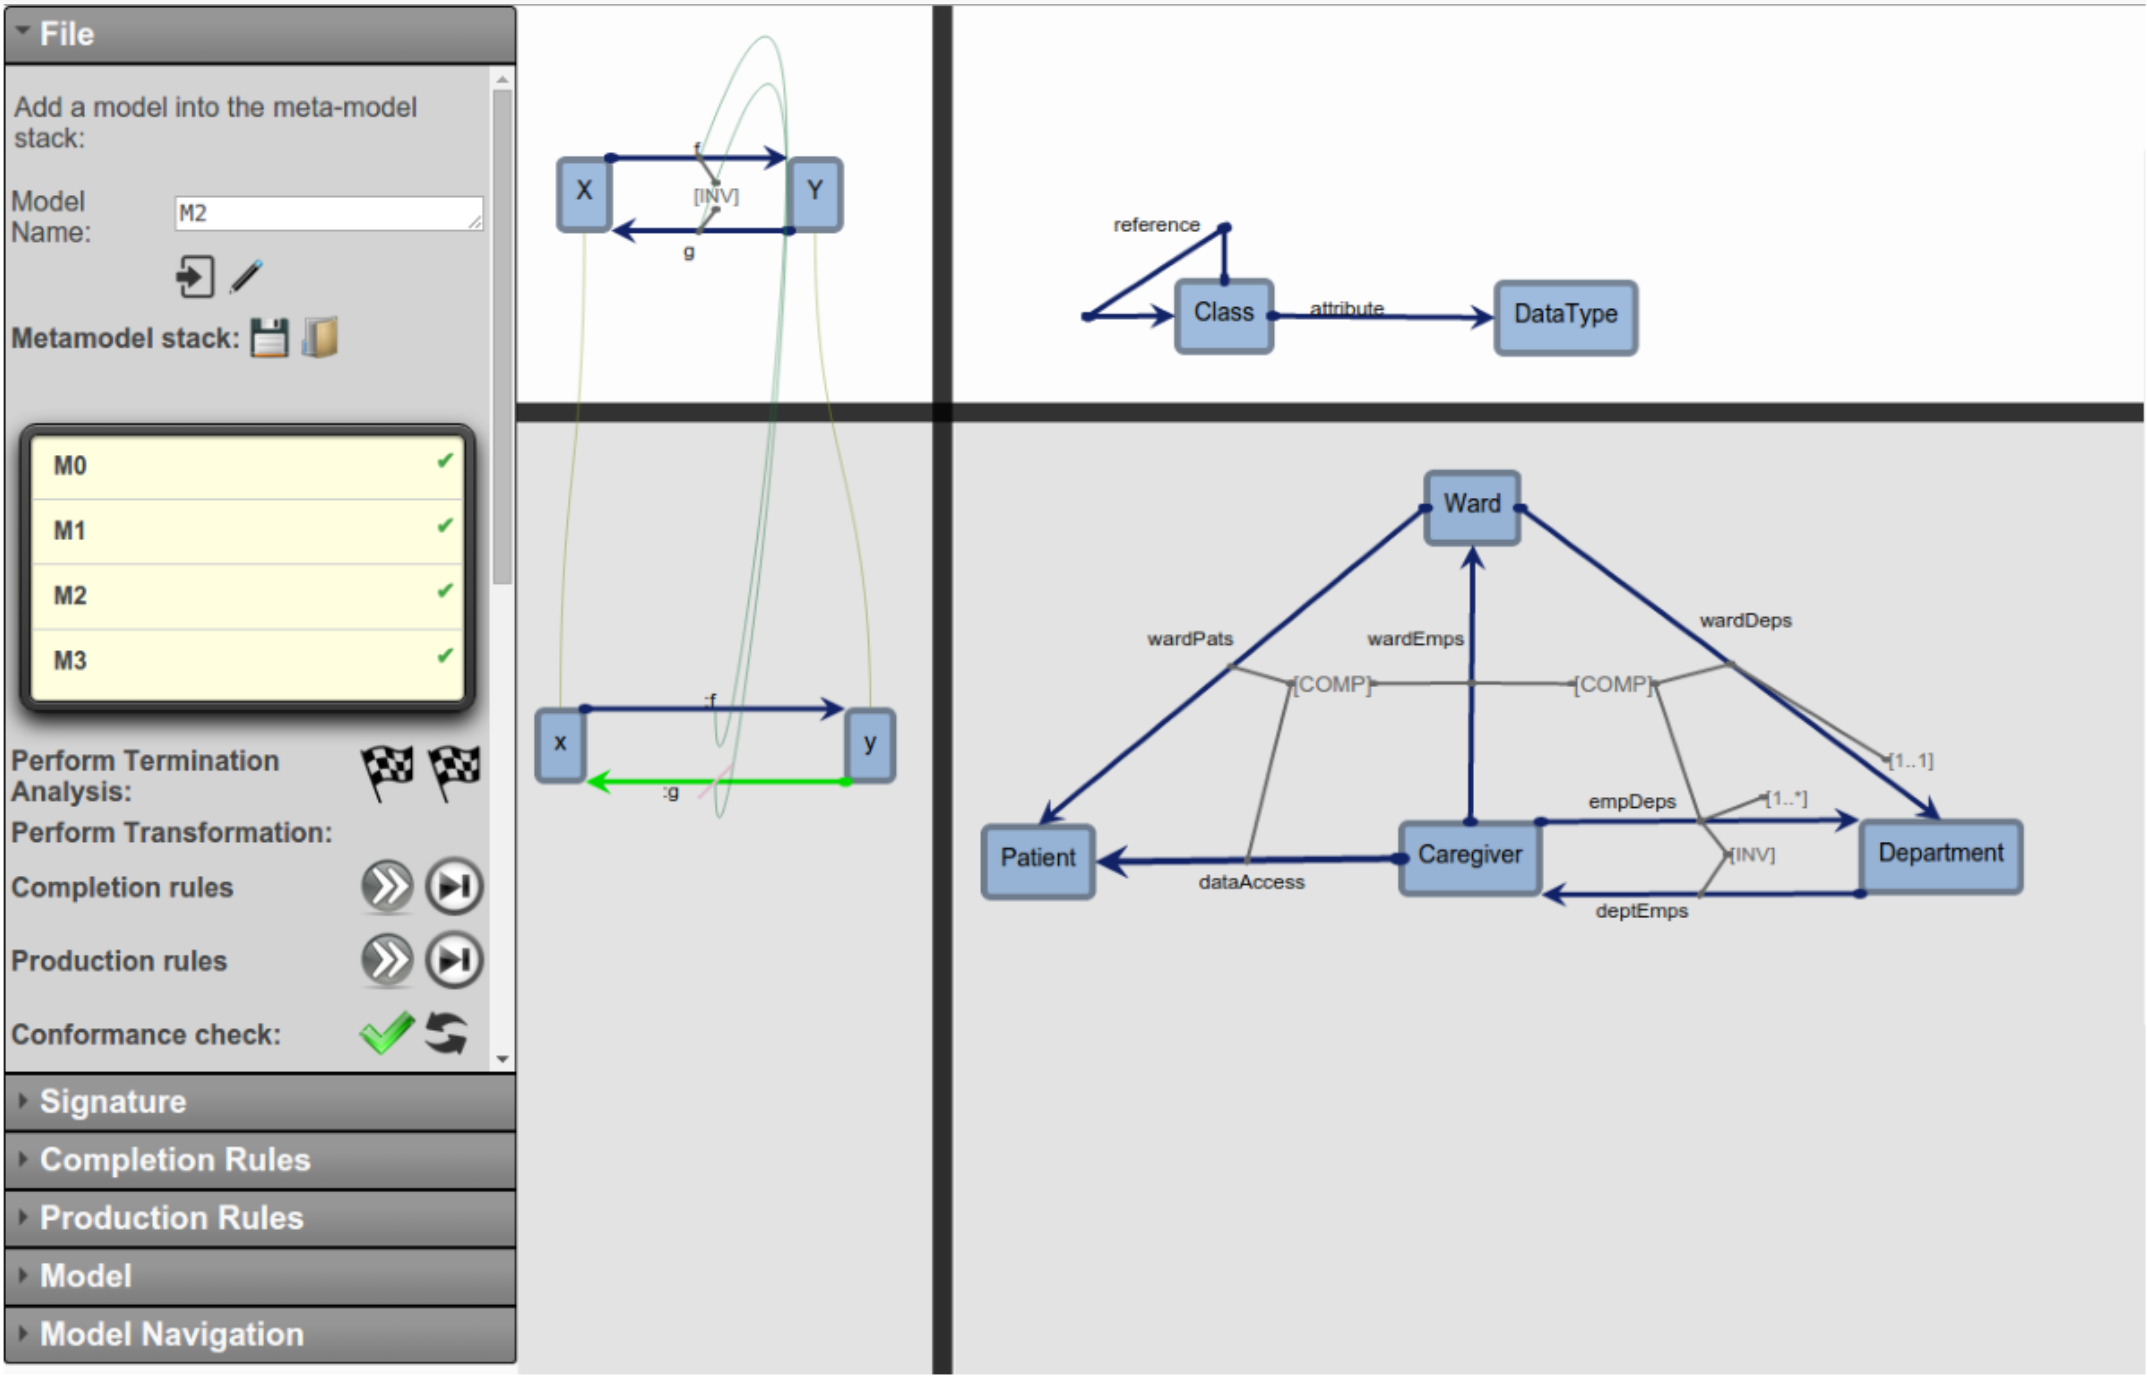
\includegraphics[width=0.8\textwidth]{webdpf.png}
	\end{center}
	\caption{Пользовательский интерфейс системы WebDPF, из~\cite{rabbi2016webdpf}}
	\label{figure:webdpf}
\end{figure}

Редактор, насколько можно судить, написан на JavaScript с AngularJS, и по сути то, к чему, наверное, стремится наш Web Modeling Project, только мы отстали примерно года на четыре. Единственная проблема WebDPF, опять-таки насколько можно судить, --- это сильная исследовательская направленность проекта, никаких упоминаний о больших моделях или содержательных инструментах моделирования для конечного пользователя в литературе не встречалось. Инструмент как будто специально писался для конференции MODELSWARD (и взял на MODELSWARD 2016 награду ``лучшая студенческая работа''). Действительно, узлы на диаграмме не могут иметь вложенных узлов, так что половину диаграмм UML и многие другие содержательные языки на WebDPF пока не сделать. Но инструмент молодой и, судя по всему, хорошо написан, так что посмотрим.

\subsection{REAL.NET}

Среда REAL.NET разрабатывается мной и группой студентов под моим руководством начиная с прошлого года с переменной активностью, при этом она ещё мало пригодна для использования, так что вряд ли её вообще можно приводить в одном списке с вышеуказанными работами. Тем не менее, краткое описание для полноты приведу, более подробно среда описана в работе~\cite{litvinov2017realnet}. REAL.NET предназначена для того, чтобы быстро создавать предметно-ориентированные языки и инструменты для них, либо автономные, либо встраиваемые в существующие .NET-приложения. Она реализует инфраструктуру для глубокого метамоделирования и (пока что) использует глубокое инстанцирование для того, чтобы распространять лингвистические свойства (такие как форма элемента, имя элемента и т.д.) по иерархии метауровней. Среда реализует иерархию метамоделей, в корне которой рефлексивная метамодель ``Core Metamodel''. Она выражается сама через себя и через код на языке программирования (F\# в нашем случае). Диаграмма этой метамодели представлена на рисунке~\ref{figure:realNetMetametamodel}.

\begin{figure}
	\begin{center}
		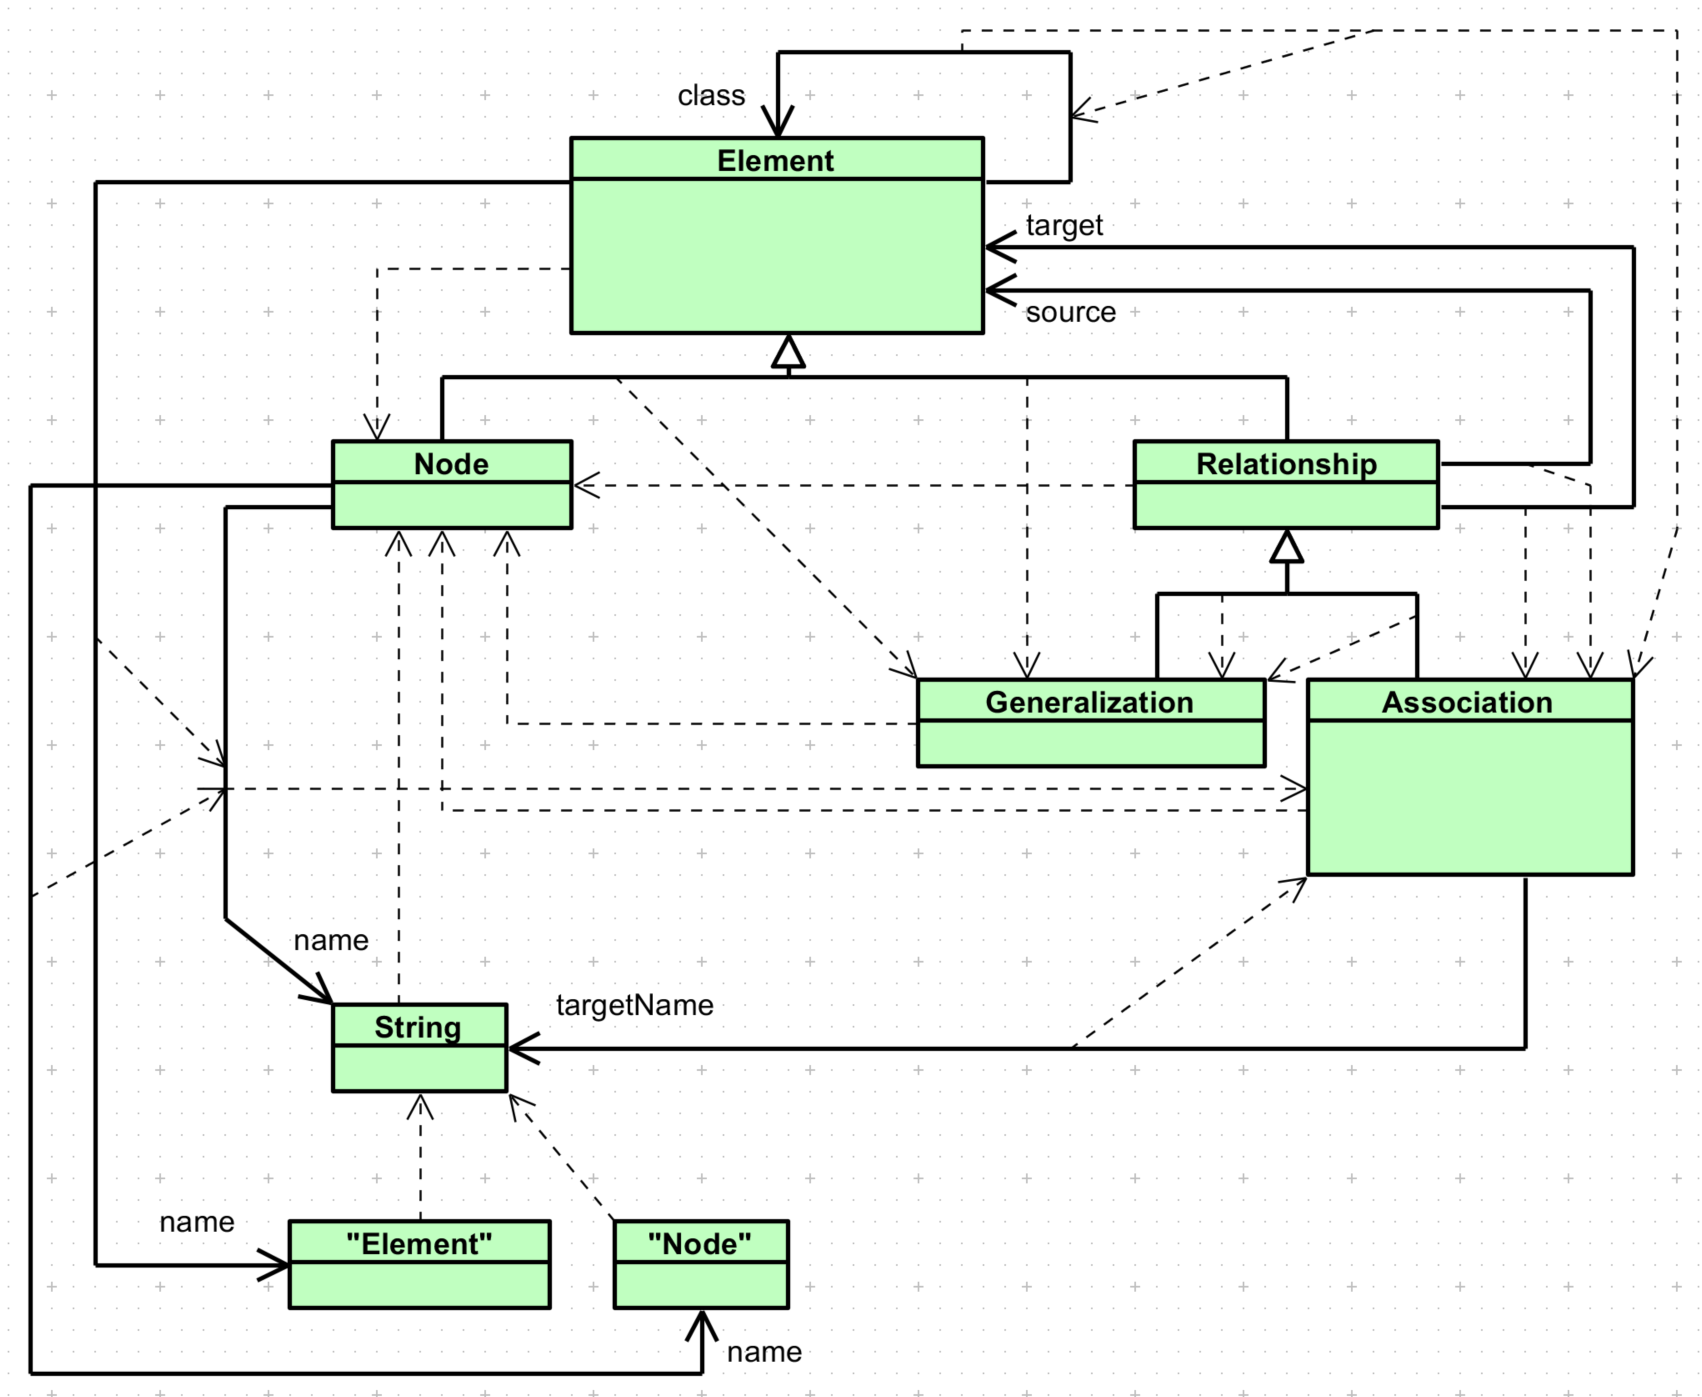
\includegraphics[width=0.9\textwidth]{realNetMetametamodel.png}
	\end{center}
	\caption{Корневая метамодель системы REAL.NET}
	\label{figure:realNetMetametamodel}
\end{figure}

Следует обратить внимание, что в корневой метамодели отсутствует даже понятие ``Атрибут'', поскольку появление атрибутов сразу влечёт появление понятий ``Тип'' и ``Значение'', что сразу усложняет метамодель примерно вдвое, а хочется по возможности минимальную метамодель в качестве корневой. Все свойства выражаются тут в виде ассоциаций с именованными концами (причём только один конец именован), все значения хранятся как строки. Поскольку эта метамодель рефлексивна, то отношения ``является экземпляром'' связывают каждый её элемент с каким-либо другим её же элементом (показано на рисунке~\ref{figure:realNetMetametamodel} пунктирными линиями).

Использовать корневую метамодель для работы с языками сложно и неэффективно, поэтому с помощью неё определена ``языковая метамодель'', которая вводит необходимые элементы метаязыка (пока обошлись только типом ``перечисление''), а с её помощью ``инфраструктурная метамодель'', которая содержит в себе уже всё необходимое для создания настоящих языков (например, понятие ``Атрибут'', понятие ``Тип'', такие важные служебные вещи, как ``Репозиторий'' и ``Модель''). Инфраструктурная метамодель также имеет отражение в коде --- ей соответствует интерфейс репозитория и её поддерживают визуальные редакторы (например, в инфраструктурной метамодели определена форма элемента, которую редакторы получают через интерфейс репозитория, чтобы рисовать элемент на сцене). В репозитории данные о модели хранятся (по крайней мере, на данный момент) в формате корневой метамодели, информация об ``инфраструктурных'' свойствах (например, атрибутах сущности) получается из репозитория исполнением запросов к ``графу'' модели. Слово ``граф'' взято в кавычки потому, что REAL.NET на самом деле позволяет соединять связями любые сущности, в том числе и связи, так что строго говоря графом не является (пример, почему это нужно, можно видеть на рисунке~\ref{figure:realNetMetametamodel}, и хочется заметить, что даже редактор UML Visual Paradigm, в котором была нарисована эта диаграмма, связи между связями поддерживает).

На данный момент реализован репозиторий с инфраструктурой метамоделей и операцией инстанцирования, редактор для Windows с использованием библиотек GraphX и WPF, и редактор для Linux с использованием MS AGL и WinForms (впрочем, редактор для Linux сейчас не поддерживается и, возможно, уже не работоспособен). Внешний вид редактора для Windows показан на рисунке~\ref{figure:realNet}.

\begin{figure}
	\begin{center}
		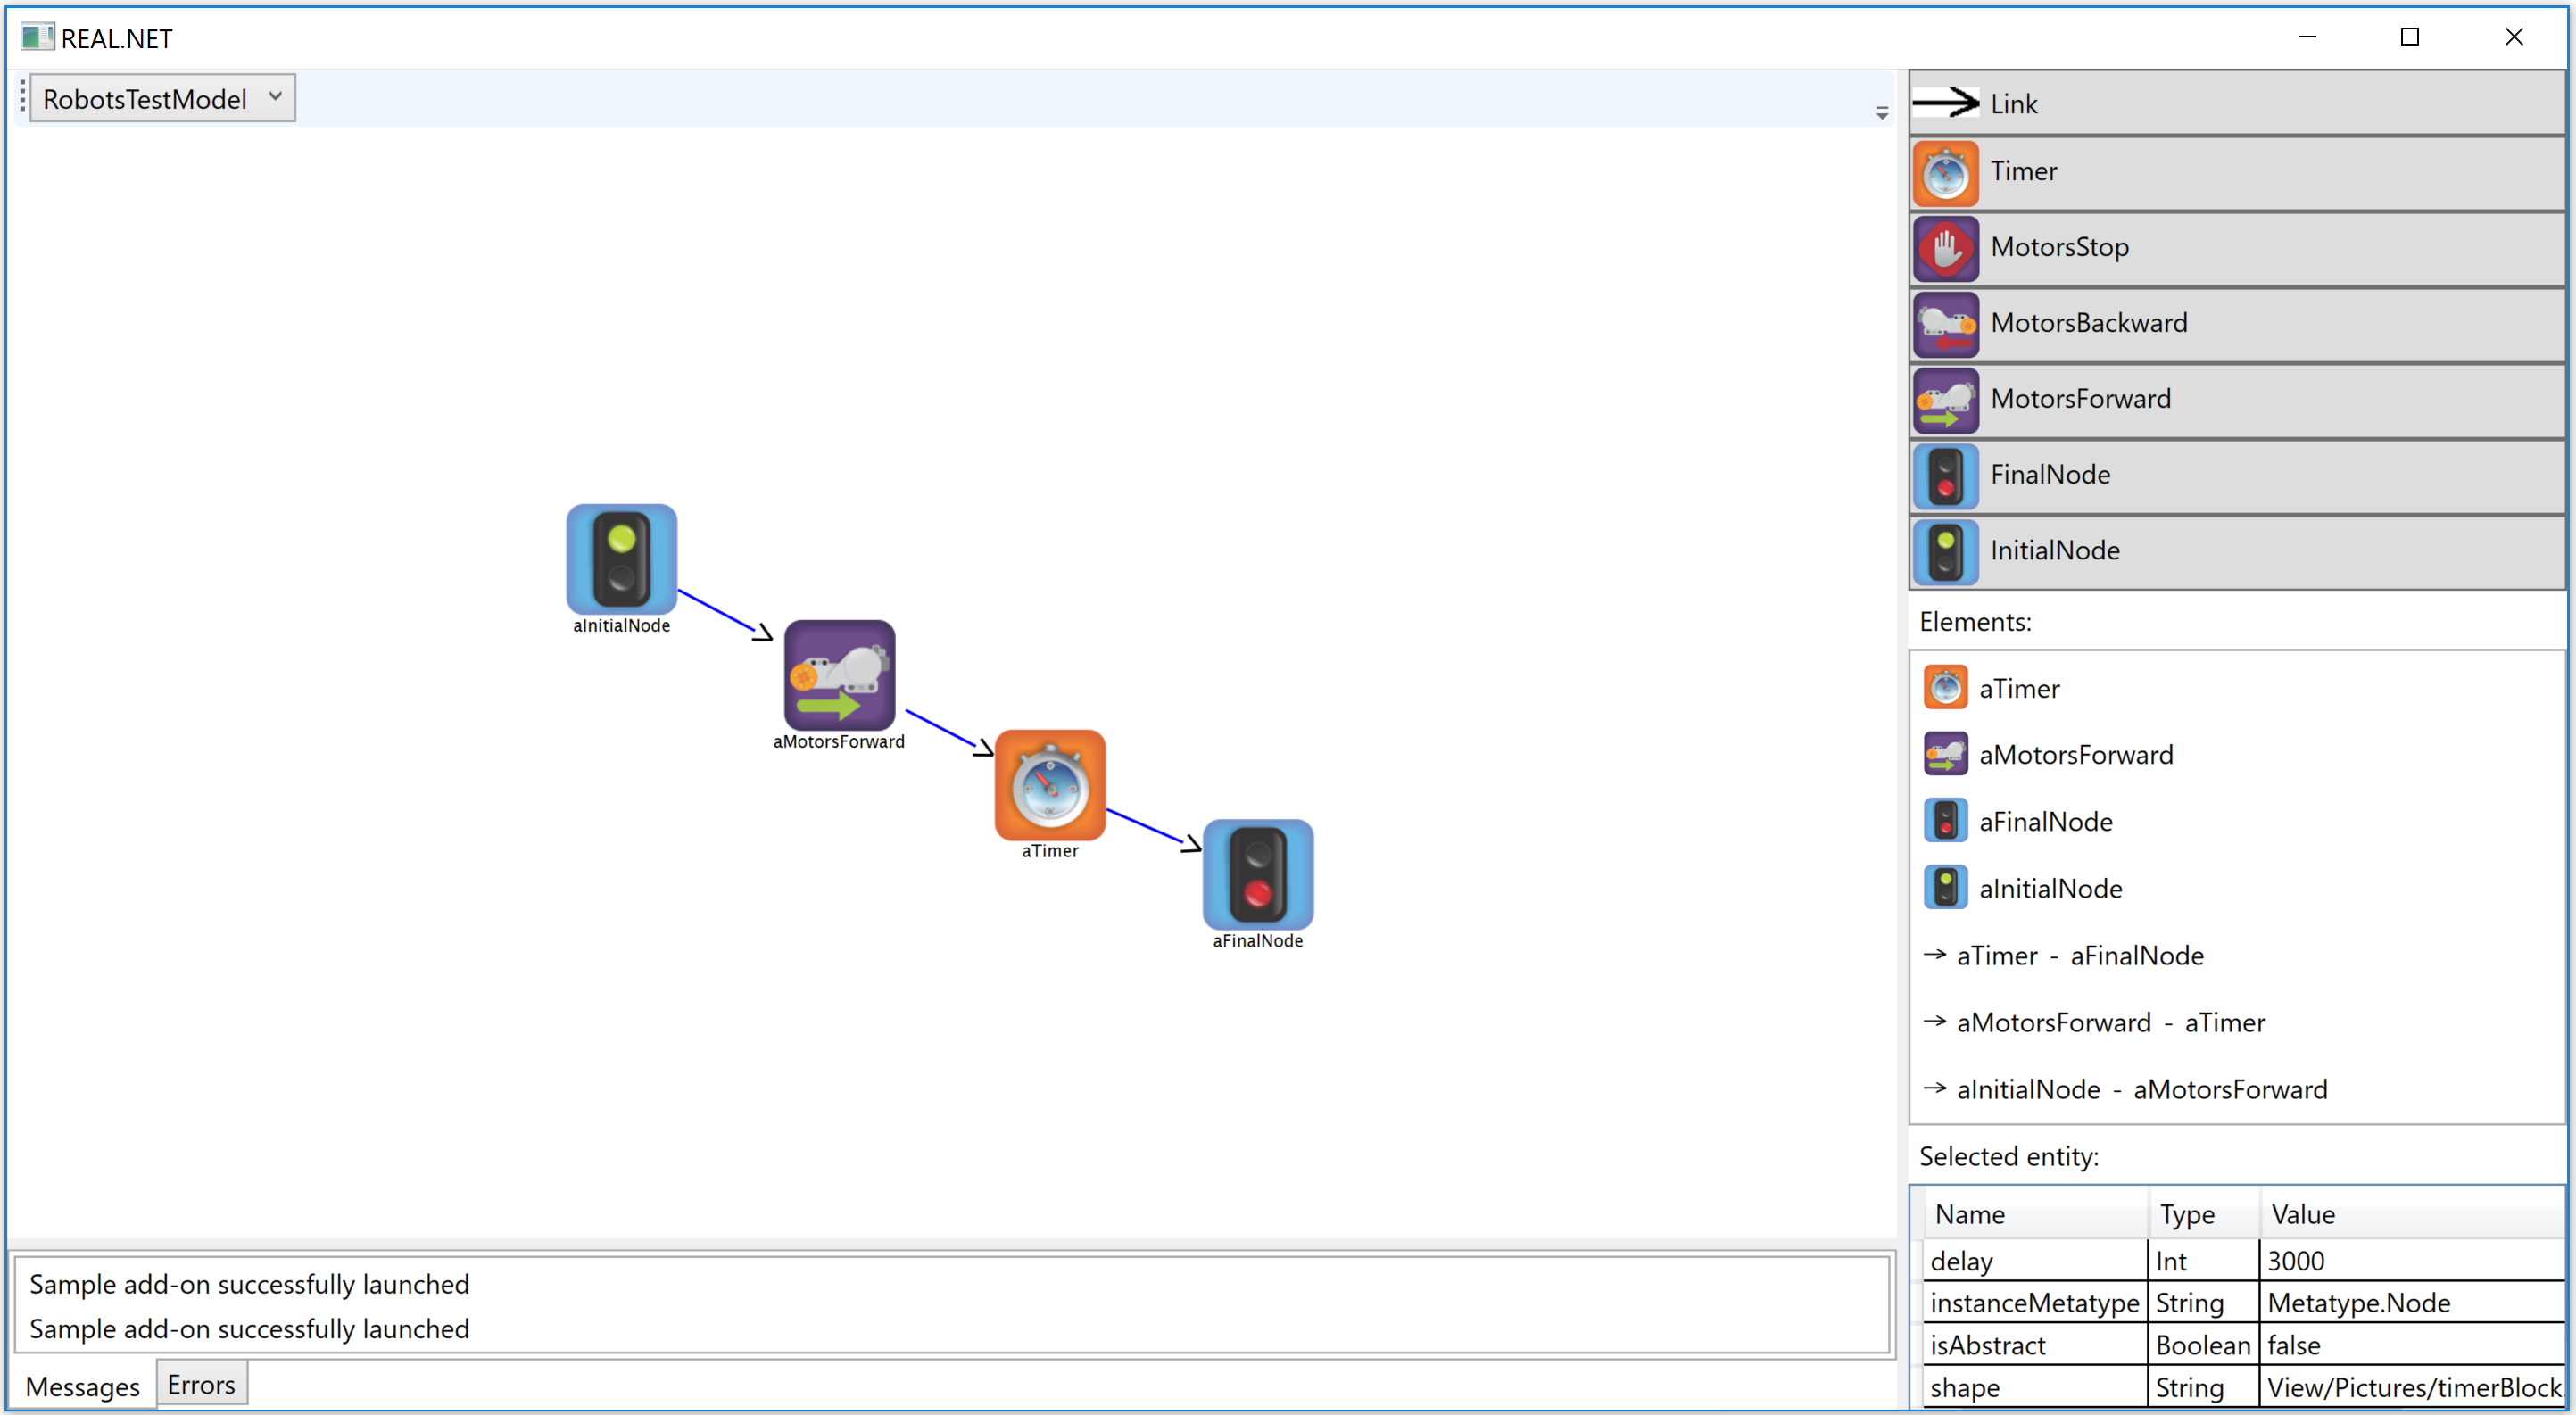
\includegraphics[width=0.9\textwidth]{realNet.png}
	\end{center}
	\caption{Пользовательский интерфейс системы REAL.NET}
	\label{figure:realNet}
\end{figure}

\section*{Заключение}

В докладе обсуждался один подход к формальному определению визуальных языков, ``глубокое метамоделирование''. Существуют и другие интересные подходы, например, паттерн ``Powertype'', описанный в работе~\cite{gonzalez2006powertype}. Попробовать их все на практике и сравнить достоинства и недостатки при создании реальных инструментов моделирования и реальных метамоделей для практически полезных языков --- интересная задача. Реализация инструмента, поддерживающего глубокое метамоделирование, уже выявила невозможность напрямую переиспользовать описанные в литературе результаты и общий недостаток информации касательно реализационных аспектов этого подхода, так что, возможно, продолжение работы с целью исследования этих аспектов и дальнейшего развития самого подхода может быть интересно мировому сообществу.

Также кажется интересным начать практическое применение разрабатываемых инструментов. Все известные мне существующие работы носят чисто академический характер, тогда как технологии должны создаваться для того, чтобы ими пользовались на практике. Поэтому сейчас в REAL.NET ведутся работы по созданию визуального языка программирования умной теплицы и симулятора квадрокоптера AirSim. Интересным направлением развития проекта кажется отработка технологии создания подобных прикладных средств и увеличение их количества, по возможности силами студентов.

\bibliographystyle{utf8gost705u}
\bibliography{deep-metamodeling-text}

\end{document}
